% Judul Dokumen
\title{Buku Tugas Akhir ITS}
\author{Musk, Elon Reeve}

% Pengaturan ukuran teks dan bentuk halaman dua sisi
\documentclass[12pt,twoside]{report}

% Pengaturan ukuran halaman dan margin
\usepackage[a4paper,top=30mm,left=30mm,right=20mm,bottom=25mm]{geometry}

% Pengaturan ukuran spasi
\usepackage[singlespacing]{setspace}

% Pengaturan detail pada file PDF
\usepackage[pdfauthor={\@author},bookmarksnumbered,pdfborder={0 0 0}]{hyperref}

% Pengaturan jenis karakter
\usepackage[utf8]{inputenc}

% Pengaturan pewarnaan
\usepackage[table,xcdraw]{xcolor}

% Pengaturan kutipan artikel
\usepackage[style=apa, backend=biber]{biblatex}

% Package lainnya
\usepackage{changepage}
\usepackage{enumitem}
\usepackage{eso-pic}
\usepackage{txfonts} % Font times
\usepackage{etoolbox}
\usepackage{graphicx}
\usepackage{lipsum}
\usepackage{longtable}
\usepackage{tabularx}
\usepackage{wrapfig}
\usepackage{multirow}

% Definisi untuk "Hati ini sengaja dikosongkan"
\patchcmd{\cleardoublepage}{\hbox{}}{
  \thispagestyle{empty}
  \vspace*{\fill}
  \begin{center}\textit{[Halaman ini sengaja dikosongkan]}\end{center}
  \vfill}{}{}

% Pengaturan penomoran halaman
\usepackage{fancyhdr}
\fancyhf{}
\renewcommand{\headrulewidth}{0pt}
\pagestyle{fancy}
\fancyfoot[LE,RO]{\thepage}
\patchcmd{\chapter}{plain}{fancy}{}{}
\patchcmd{\chapter}{empty}{plain}{}{}

% Command untuk bulan
\newcommand{\MONTH}{%
  \ifcase\the\month
  \or Januari% 1
  \or Februari% 2
  \or Maret% 3
  \or April% 4
  \or Mei% 5
  \or Juni% 6
  \or Juli% 7
  \or Agustus% 8
  \or September% 9
  \or Oktober% 10
  \or November% 11
  \or Desember% 12
  \fi}
\newcommand{\ENGMONTH}{%
  \ifcase\the\month
  \or January% 1
  \or February% 2
  \or March% 3
  \or April% 4
  \or May% 5
  \or June% 6
  \or July% 7
  \or August% 8
  \or September% 9
  \or October% 10
  \or November% 11
  \or December% 12
  \fi}

% Pengaturan format judul bab
\usepackage{titlesec}
\titleformat{\chapter}[display]{\bfseries\Large}{BAB \centering\Roman{chapter}}{0ex}{\vspace{0ex}\centering}
\titleformat{\section}{\bfseries\large}{\MakeUppercase{\thesection}}{1ex}{\vspace{1ex}}
\titleformat{\subsection}{\bfseries\large}{\MakeUppercase{\thesubsection}}{1ex}{}
\titleformat{\subsubsection}{\bfseries\large}{\MakeUppercase{\thesubsubsection}}{1ex}{}
\titlespacing{\chapter}{0ex}{0ex}{4ex}
\titlespacing{\section}{0ex}{1ex}{0ex}
\titlespacing{\subsection}{0ex}{0.5ex}{0ex}
\titlespacing{\subsubsection}{0ex}{0.5ex}{0ex}

% Atur variabel berikut sesuai namanya

% nama
\newcommand{\name}{Hans Fahrezi}
\newcommand{\authorname}{Fahrezi, Hans}
\newcommand{\nickname}{Hans}
\newcommand{\advisor}{Reza Fuad Rachmadi, S.T., M.T., Ph.D}
\newcommand{\coadvisor}{Dr. Supeno Mardi Susiki Nugroho, S.T., M.T.}
\newcommand{\examinerone}{Dr. I Ketut Eddy Purnama., S.T., M.T}
\newcommand{\examinertwo}{Ir. Hanny Budinugroho, S.T., M.T}
% \newcommand{\examinerthree}{Mochamad Hariadi, S.T., M.Sc., Ph.D}
\newcommand{\headofdepartment}{Dr. Supeno Mardi Susiki Nugroho, S.T., M.T}

% identitas
\newcommand{\nrp}{0721 19 4000 0043}
\newcommand{\advisornip}{19850403 201212 1 001}
\newcommand{\coadvisornip}{19700313 199512 1 001}
\newcommand{\examineronenip}{19690730199512 1 001}
\newcommand{\examinertwonip}{19610706198701 1 001}
% \newcommand{\examinerthreenip}{199691209199703 1 002}
\newcommand{\headofdepartmentnip}{19700313 199512 1 001}

% judul
\newcommand{\tatitle}{RE-IDENTIFIKASI MOBIL PADA CITRA KAMERA PENGAWAS LALU LINTAS MENGGUNAKAN \emph{SWIN TRANSFORMER}}
\newcommand{\engtatitle}{CAR RE-IDENTIFICATION ON TRAFFIC MONITORING CAMERA IMAGES USING SWIN TRANSFORMER}

% tempat
\newcommand{\place}{Surabaya}

% jurusan
\newcommand{\studyprogram}{Teknik Komputer}
\newcommand{\engstudyprogram}{Computer Engineering}

% fakultas
\newcommand{\faculty}{Teknologi Elektro dan Informatika Cerdas}
\newcommand{\engfaculty}{Intelligent Electrical and Informatics Technology}

% singkatan fakultas
\newcommand{\facultyshort}{FTEIC}
\newcommand{\engfacultyshort}{FTEIC}

% departemen
\newcommand{\department}{Teknik Komputer}
\newcommand{\engdepartment}{Computer Engineering}

% kode mata kuliah
\newcommand{\coursecode}{EC224801}


% Tambahkan format tanda hubung yang benar di sini
\hyphenation{
  ro-ket
  me-ngem-bang-kan
  per-hi-tu-ngan
  tek-no-lo-gi
  me-la-ku-kan
  ber-so-si-al-i-sa-si
}

% Menambahkan resource daftar pustaka
\addbibresource{pustaka/pustaka.bib}

% Pengaturan format potongan kode
\usepackage{listings}
\definecolor{comment}{RGB}{0,128,0}
\definecolor{string}{RGB}{255,0,0}
\definecolor{keyword}{RGB}{0,0,255}
\lstdefinestyle{codestyle}{
  commentstyle=\color{comment},
  stringstyle=\color{string},
  keywordstyle=\color{keyword},
  basicstyle=\footnotesize\ttfamily,
  numbers=left,
  numberstyle=\tiny,
  numbersep=5pt,
  frame=lines,
  breaklines=true,
  prebreak=\raisebox{0ex}[0ex][0ex]{\ensuremath{\hookleftarrow}},
  showstringspaces=false,
  upquote=true,
  tabsize=2,
}
\lstset{style=codestyle}

% Isi keseluruhan dokumen
\begin{document}

% Sampul luar Bahasa Indonesia
\newcommand\covercontents{sampul/konten-id.tex}
\AddToShipoutPictureBG*{
  \AtPageLowerLeft{
    % Ubah nilai berikut jika posisi horizontal background tidak sesuai
    \hspace{-3.25mm}

    % Ubah nilai berikut jika posisi vertikal background tidak sesuai
    \raisebox{0mm}{
      
\includegraphics[width=\paperwidth,height=\paperheight]{sampul/gambar/sampul-luar.png}
    }
  }
}

% Menyembunyikan nomor halaman
\thispagestyle{empty}

% Pengaturan margin untuk menyesuaikan konten sampul
\newgeometry{
  top=55mm,
  left=30mm,
  right=20mm,
  bottom=20mm
}

\begin{flushleft}

  % Pemilihan font sans serif
  \sffamily

  % Pemilihan warna font putih
  \color{white}

  % Pemilihan font bold
  \fontseries{bx}
  \selectfont
  \begin{spacing}{1.5}
    \input{\covercontents}
  \end{spacing}

\end{flushleft}

\restoregeometry


% Atur ulang penomoran halaman
\setcounter{page}{1}

% Sampul dalam Bahasa Indonesia
\renewcommand\covercontents{sampul/konten-id.tex}
\AddToShipoutPictureBG*{
  \AtPageLowerLeft{
    % Ubah nilai berikut jika posisi horizontal background tidak sesuai
    \hspace{-4mm}

    % Ubah nilai berikut jika posisi vertikal background tidak sesuai
    \raisebox{0mm}{
      
\includegraphics[width=\paperwidth,height=\paperheight]{sampul/gambar/sampul-luar-tipis.png}
    }
  }
}

% Menyembunyikan nomor halaman
\thispagestyle{empty}

% Pengaturan margin untuk menyesuaikan konten sampul
\newgeometry{
  top=65mm,
  left=30mm,
  right=30mm,
  bottom=20mm
}

\begin{flushleft}

  % Pemilihan font sans serif
  \sffamily

  % Pemilihan font bold
  \fontseries{bx}
  \selectfont
  \begin{spacing}{1.5}
    \input{\covercontents}
  \end{spacing}

\end{flushleft}

\restoregeometry

\clearpage
\cleardoublepage

% Sampul dalam Bahasa Inggris
\renewcommand\covercontents{sampul/konten-en.tex}
\AddToShipoutPictureBG*{
  \AtPageLowerLeft{
    % Ubah nilai berikut jika posisi horizontal background tidak sesuai
    \hspace{-4mm}

    % Ubah nilai berikut jika posisi vertikal background tidak sesuai
    \raisebox{0mm}{
      
\includegraphics[width=\paperwidth,height=\paperheight]{sampul/gambar/sampul-luar-tipis.png}
    }
  }
}

% Menyembunyikan nomor halaman
\thispagestyle{empty}

% Pengaturan margin untuk menyesuaikan konten sampul
\newgeometry{
  top=65mm,
  left=30mm,
  right=30mm,
  bottom=20mm
}

\begin{flushleft}

  % Pemilihan font sans serif
  \sffamily

  % Pemilihan font bold
  \fontseries{bx}
  \selectfont
  \begin{spacing}{1.5}
    \input{\covercontents}
  \end{spacing}

\end{flushleft}

\restoregeometry

\cleardoublepage

% Pengaturan ukuran indentasi paragraf
\setlength{\parindent}{2em}

% Pengaturan ukuran spasi paragraf
\setlength{\parskip}{1ex}

% Lembar pengesahan
\begin{center}
  \large
  \textbf{LEMBAR PENGESAHAN}
\end{center}

% Menyembunyikan nomor halaman
\thispagestyle{empty}

\begin{center}
  \textbf{\tatitle{}}
\end{center}

\begingroup
% Pemilihan font ukuran small
\small

\begin{center}
  \textbf{TUGAS AKHIR}
  \\Diajukan untuk memenuhi salah satu syarat \\
  memperoleh gelar Sarjana Teknik pada \\
  Program Studi S-1 \studyprogram{} \\
  Departemen \department{} \\
  Fakultas \faculty{} \\
  Institut Teknologi Sepuluh Nopember
\end{center}

\begin{center}
  Oleh: \textbf{\name{}}
  \\NRP. \nrp{}
\end{center}

\begin{center}
  Disetujui oleh Tim Penguji Tugas Akhir:
\end{center}

\begingroup
% Menghilangkan padding
\setlength{\tabcolsep}{0pt}

\noindent
\begin{tabularx}{\textwidth}{X l}
  \advisor{}               & (Pembimbing I)                      \\
  NIP: \advisornip{}       &                                     \\
                           & ................................... \\
                           &                                     \\
                           &                                     \\
  \coadvisor{}             & (Pembimbing II)                     \\
  NIP: \coadvisornip{}     &                                     \\
                           & ................................... \\
                           &                                     \\
                           &                                     \\
  \examinerone{}.          & (Penguji I)                         \\
  NIP: \examineronenip{}   &                                     \\
                           & ................................... \\
                           &                                     \\
                           &                                     \\
  \examinertwo{}.          & (Penguji II)                        \\
  NIP: \examinertwonip{}   &                                     \\
                           & ................................... \\
  %                          &                                     \\
  %                          &                                     \\
  % \examinerthree{}.        & (Penguji III)                       \\
  % NIP: \examinerthreenip{} &                                     \\
  %                          & ................................... \\
\end{tabularx}
\endgroup

\begin{center}
  Mengetahui, \\
  Kepala Departemen \department{} \facultyshort{} - ITS\\

  \vspace{8ex}

  \underline{\headofdepartment{}.} \\
  NIP. \headofdepartmentnip{}
\end{center}

\begin{center}
  \textbf{\MakeUppercase{\place{}}\\\MONTH{}, \the\year{}}
\end{center}
\endgroup

\cleardoublepage
\begin{center}
  \large
  \textbf{APPROVAL SHEET}
\end{center}

% Menyembunyikan nomor halaman
\thispagestyle{empty}

\begin{center}
  \textbf{\engtatitle{}}
\end{center}

\begingroup
% Pemilihan font ukuran small
\small

\begin{center}
  \textbf{FINAL PROJECT}
  \\Submitted to fulfill one of the requirements \\
  for obtaining a degree Bachelor of Engineering at \\
  Undergraduate Study Program of \engstudyprogram{} \\
  Department of \engdepartment{} \\
  Faculty of \engfaculty{} \\
  Sepuluh Nopember Institute of Technology
\end{center}

\begin{center}
  By: \textbf{\name{}}
  \\NRP. \nrp{}
\end{center}

\begin{center}
  Approved by Final Project Examiner Team:
\end{center}

\begingroup
% Menghilangkan padding
\setlength{\tabcolsep}{0pt}

\noindent
\begin{tabularx}{\textwidth}{X l}
  \advisor{}               & (Advisor I)                         \\
  NIP: \advisornip{}       &                                     \\
                           & ................................... \\
                           &                                     \\
                           &                                     \\
  \coadvisor{}             & (Co-Advisor II)                     \\
  NIP: \coadvisornip{}     &                                     \\
                           & ................................... \\
                           &                                     \\
                           &                                     \\
  \examinerone{}.          & (Examiner I)                        \\
  NIP: \examineronenip{}   &                                     \\
                           & ................................... \\
                           &                                     \\
                           &                                     \\
  \examinertwo{}.          & (Examiner II)                       \\
  NIP: \examinertwonip{}   &                                     \\
                           & ................................... \\
  %                          &                                     \\
  %                          &                                     \\
  % \examinerthree{}.        & (Examiner III)                      \\
  % NIP: \examinerthreenip{} &                                     \\
  %                          & ................................... \\
\end{tabularx}
\endgroup


\begin{center}
  Acknowledged, \\
  Head of \engdepartment{} Department \engfacultyshort{} - ITS \\

  \vspace{8ex}

  \underline{\headofdepartment{}.} \\
  NIP. \headofdepartmentnip{}
\end{center}

\begin{center}
  \textbf{\MakeUppercase{\place{}}\\\ENGMONTH{}, \the\year{}}
\end{center}
\endgroup

\cleardoublepage

% Pernyataan keaslian
\begin{center}
  \large
  \textbf{PERNYATAAN ORISINALITAS}
\end{center}

% Menyembunyikan nomor halaman
\thispagestyle{empty}

\vspace{2ex}

% Ubah paragraf-paragraf berikut sesuai dengan yang ingin diisi pada pernyataan keaslian

\noindent Yang bertanda tangan dibawah ini:

\noindent\begin{tabularx}{\textwidth}{l l X}
                         &   &                            \\
  Nama Mahasiswa / NRP   & : & \name{} / \nrp{}           \\
  Departemen             & : & \department{}              \\
  Dosen Pembimbing / NIP & : & \advisor{} / \advisornip{} \\
                         &   &                            \\
\end{tabularx}

Dengan ini menyatakan bahwa Tugas Akhir dengan judul "\tatitle{}" adalah hasil karya sendiri, berfsifat orisinal, dan ditulis dengan mengikuti kaidah penulisan ilmiah.

Bilamana di kemudian hari ditemukan ketidaksesuaian dengan pernyataan ini, maka saya bersedia menerima sanksi sesuai dengan ketentuan yang berlaku di Institut Teknologi Sepuluh Nopember.

\vspace{8ex}

\noindent\begin{tabularx}{\textwidth}{X l}
                     & \place{}, \ENGMONTH{} \the\year{} \\
                     &                                   \\
  Mengetahui         &                                   \\
  Dosen Pembimbing   & Mahasiswa                         \\
                     &                                   \\
                     &                                   \\
                     &                                   \\
                     &                                   \\
                     &                                   \\
  \advisor{}         & \name{}                           \\
  NIP. \advisornip{} & NRP. \nrp{}                       \\
\end{tabularx}

\cleardoublepage
\begin{center}
  \large
  \textbf{STATEMENT OF ORIGINALITY}
\end{center}

% Menyembunyikan nomor halaman
\thispagestyle{empty}

\vspace{2ex}

% Ubah paragraf-paragraf berikut sesuai dengan yang ingin diisi pada pernyataan keaslian

\noindent The undersigned below:

\noindent\begin{tabularx}{\textwidth}{l l X}
                        &   &                            \\
  Name of student / NRP & : & \name{} / \nrp{}           \\
  Department            & : & \engdepartment{}           \\
  Advisor / NIP         & : & \advisor{} / \advisornip{} \\
                        &   &                            \\
\end{tabularx}

Hereby declared that the Final Project with the title of "\engtatitle{}" is the result of my own work, is original, and is written by following the rules of scientific writing.

If in future there is a discrepancy with this statement, then I am willing to accept sanctions in accordance with provisions that apply at Sepuluh Nopember Institute of Technology.

\vspace{8ex}

\noindent\begin{tabularx}{\textwidth}{X l}
                     & \place{}, \ENGMONTH{} \the\year{} \\
                     &                                   \\
  Acknowledged       &                                   \\
  Advisor            & Student                           \\
                     &                                   \\
                     &                                   \\
                     &                                   \\
                     &                                   \\
                     &                                   \\
  \advisor{}         & \name{}                           \\
  NIP. \advisornip{} & NRP. \nrp{}                       \\
\end{tabularx}
\cleardoublepage

% Nomor halaman pembuka dimulai dari sini
\pagenumbering{roman}

% Abstrak Bahasa Indonesia
\begin{center}
  \large\textbf{ABSTRAK}
\end{center}

\addcontentsline{toc}{chapter}{ABSTRAK}

\vspace{2ex}

\begingroup
% Menghilangkan padding
\setlength{\tabcolsep}{0pt}

\noindent
\begin{tabularx}{\textwidth}{l >{\centering}m{2em} X}
  Nama Mahasiswa    & : & \name{}         \\

  Judul Tugas Akhir & : & \tatitle{}      \\

  Pembimbing        & : & 1. \advisor{}   \\
                    &   & 2. \coadvisor{} \\
\end{tabularx}
\endgroup

% Ubah paragraf berikut dengan abstrak dari tugas akhir
Indonesia memiliki skor kriminalitas yang cukup tinggi di dunia pada tahun 2021. \linebreak 
Berdasarkan data Criminal Scores yang dibuat oleh Global Initiative Against Transnational 
Organized Crime (GITOC), Indonesia tercatat memiliki skor 6.38 dan berada di urutan 25 dari 193
negara yang terdaftar di PBB. Pada tahun 2020, angka kejahatan yang terjadi di Indonesia sebanyak 
247.218 kasus dengan Sumatera Utara memiliki 32.990 kasus kejahatan. Beberapa kasus kejahatan 
yang terjadi sering menggunakan kendaraan khususnya mobil sebagai alat untuk
membantu pelaku dalam melaksanakan tindakannya. Dengan berkembangnya teknologi pada
saat ini, melakukan pelacakan mobil pelaku dapat menggunakan sebuah model re-identifikasi.
Model re-identifikasi mobil ini dapat mengidentifikasi mobil pada sebuah tangkapan citra
berdasarkan data mobil yang dimaksud. Pada penelitian tugas akhir ini, dikembangkan sebuah
model re-identifikasi menggunakan metode terbaru yaitu Swin Transformer. Swin Transformer
merupakan sebuah arsitektur terbaru yang dikembangkan dari arsitektur Convolutional Neural
Network (CNN) dan Vision Transformer, sehingga memiliki kelebihan dibandingkan arsitektur
yang sudah lama ada. Dari pengembangan model reidentifikasi mobil dengan metode Swin
Transformer, diharapkan dapat mempermudah dalam pelacakan dan pemecahan kasus yang ditangani 
oleh polisi.

% Ubah kata-kata berikut dengan kata kunci dari tugas akhir
Kata Kunci: kriminalitas, re-identifikasi, \emph{Swin Transformer}, VRIC.

\cleardoublepage

% Abstrak Bahasa Inggris
\begin{center}
  \large\textbf{ABSTRACT}
\end{center}

\addcontentsline{toc}{chapter}{ABSTRACT}

\vspace{2ex}

\begingroup
% Menghilangkan padding
\setlength{\tabcolsep}{0pt}

\noindent
\begin{tabularx}{\textwidth}{l >{\centering}m{3em} X}
  \emph{Name}     & : & \name{}         \\

  \emph{Title}    & : & \engtatitle{}   \\

  \emph{Advisors} & : & 1. \advisor{}   \\
                  &   & 2. \coadvisor{} \\
\end{tabularx}
\endgroup

% Ubah paragraf berikut dengan abstrak dari tugas akhir dalam Bahasa Inggris
\emph{Indonesia has a high crime score in the world in 2021. Based on Criminal Scores data
created by Global Initiative Against Transnational Organized Crime (GITOC), Indonesia is
recorded as having a score of 6.38 and ranked 25th out of 193 countries that registered at United
Nations (UN). In 2020, number of crimes that occurred in Indonesia was 247.218 cases with
North Sumatera having 32.990 crime cases. Some crime cases that occur often use vehicles,
especially cars, as a tool to assist perpetrator in carrying out their actions. With the development 
of technology at this time, tracking the perpetrator's car can use a re-identification model.
This car re-identification model can identify cars in an image capture based on the car's data.
In this final project research, a re-identification model was developed using the latest method,
and that's Swin Transformer. Swin Transformer is the latest architecture developed from Convolutional 
Neural Network (CNN) and Vision Transformer architectures, so it has advantages
over the old architectures. From this development of the car re-identification model using Swin
Transformer, hopes that it will make it easier to track and solve cases handled by the police.}

% Ubah kata-kata berikut dengan kata kunci dari tugas akhir dalam Bahasa Inggris
\emph{Keywords}: \emph{Criminality}, \emph{Re-identification}, \emph{Swin Transformer}, \emph{VRIC}.

\cleardoublepage

% Kata pengantar
\begin{center}
  \Large
  \textbf{KATA PENGANTAR}
\end{center}

\addcontentsline{toc}{chapter}{KATA PENGANTAR}

\vspace{2ex}

% Ubah paragraf-paragraf berikut dengan isi dari kata pengantar

Puji dan syukur kehadirat \lipsum[1][1-5]

Penelitian ini disusun dalam rangka \lipsum[2][1-5]
Oleh karena itu, penulis mengucapkan terima kasih kepada:

\begin{enumerate}[nolistsep]

  \item Keluarga, Ibu, Bapak dan Saudari tercinta yang selalu memberikan dukungan spiritual, moral, maupun 
  material dalam penyusunan penelitian ini.

  \item Bapak Dr. Supeno Mardi Susiki Nugroho, ST., MT., selaku Kepala Departemen Teknik Komputer, Fakultas 
  Teknologi Elektro dan Informatika Cerdas, Institut Teknologi Sepuluh Nopember Surabaya.

  \item Bapak Reza Fuad Rachmadi, ST., MT., Ph.D., selaku dosen pembimbing I dan Bapak Dr. Supeno Mardi 
  Susiki Nugroho, ST., MT., selaku dosen pembimbing II yang selalu memberikan arahan, bimbingan, dan semangat 
  selama mengerjakan penelitian Tugas Akhir ini.

\end{enumerate}

Akhir kata, semoga \lipsum[6][1-8]

\begin{flushright}
  \begin{tabular}[b]{c}
    \place{}, \MONTH{} \the\year{} \\
    \\
    \\
    \\
    \\
    \name{}
  \end{tabular}
\end{flushright}

\cleardoublepage

% Daftar isi
\renewcommand*\contentsname{DAFTAR ISI}
\addcontentsline{toc}{chapter}{\contentsname}
\tableofcontents
\cleardoublepage

% Daftar gambar
\renewcommand*\listfigurename{DAFTAR GAMBAR}
\addcontentsline{toc}{chapter}{\listfigurename}
\listoffigures
\cleardoublepage

% Daftar tabel
\renewcommand*\listtablename{DAFTAR TABEL}
\addcontentsline{toc}{chapter}{\listtablename}
\listoftables
\cleardoublepage

% Nomor halaman isi dimulai dari sini
\pagenumbering{arabic}

% Bab 1 pendahuluan
\chapter{PENDAHULUAN}
\label{chap:pendahuluan}

% Ubah bagian-bagian berikut dengan isi dari pendahuluan
\section{Latar Belakang}
\label{sec:latarbelakang}

Indonesia memiliki skor kriminalitas yang cukup tinggi di dunia pada tahun 2021. \linebreak
Berdasarkan data \emph{Criminal Scores} yang dibuat oleh \emph{Global Initiative Against Transnational Organized Crime} 
(GITOC), Indonesia tercatat memiliki skor 6.38 dan berada di urutan 25 dari 193 negara yang 
terdaftar di PBB\parencite{Gitoc2021}. Pada tahun 2020, angka kejahatan yang terjadi di Indonesia 
sebanyak 247.218 kasus dengan Sumatera Utara memiliki 32.990 kasus kejahatan\parencite{Bpskriminal2021}.
Beberapa kasus kejahatan yang terjadi sering menggunakan kendaraan sebagai alat untuk membantu pelaku 
dalam melaksanakan tindakannya.

Mobil yang digunakan di Indonesia diproduksi oleh merek dan perusahaan yang berbeda-beda 
dan setiap tipe yang diproduksi memiliki ciri khasnya masing-masing. Ciri khas ini dapat 
berupa bentuk badan kendaraan, jenis kendaraan, warna, serta ukuran. Ciri khas inilah 
yang dapat membantu mengidentifikasi tipe satu dengan lainnya.

\begin{figure}[ht]
      \centering
      % Nama dari file gambar yang diinputkan
      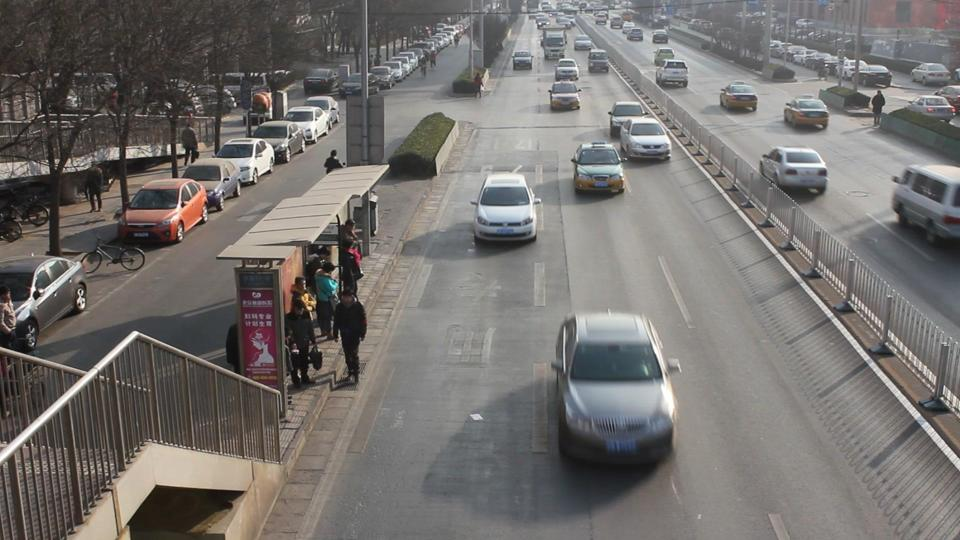
\includegraphics[scale=0.3]{gambar/Mobil.jpg}
      % Keterangan gambar yang diinputkan
      \caption{Lalu lintas dari rekaman CCTV}
      % Label referensi dari gambar yang diinputkan
      \label{fig:RekamanCCTV}
\end{figure}

Ciri khas yang dimiliki pada tiap tipe mobil inilah yang dapat membantu dalam melakukan 
re-identifikasi menggunakan metode Swin Transformer. Swin transformer merupakan 
pengembangan arsitektur Convolutional Neural Network (CNN) dan Vision Transformer yang 
baru. Swin Transformer memiliki kelebihan yang cukup menguntungkan jika dibandingkan 
dengan Vision Transformer, dimana Swin Transformer dapat memproses dan mengidentifikasi 
citra yang ditangkap dalam keadaan blur, resolusi yang kecil, dan pencahayaan yang tidak 
sempurna. Hasil yang diberikan oleh Swin Transformer lebih efisien dan akurasinya lebih tinggi.

Oleh karena itu, penulis merasa metode Swin Transformer dapat digunakan untuk membantu menangani 
kasus kejahatan. Dengan diaplikasikannya Swin Transformer pada rekaman cctv, maka dapat mempermudah 
proses pemecahan kasus kejahatan dimana kendaraan yang digunakan pelaku dapat di re-identifikasi 
dan dilacak menggunakan rekaman cctv di sekitar tempat kejadian perkara.

\section{Permasalahan}
\label{sec:permasalahan}

Dalam proses re-identifikasi mobil, sering kali terjadi kesalahan dalam melakukan re-identifikasi.
Gambar yang kurang jelas karena dalam kondisi lingkungan dengan pencahayaan yang tidak ideal,
resolusi dari gambar yang cukup kecil, serta adanya blur ketika proses pengambilan gambar, membuat model re-identifikasi
yang sudah ada saat ini belum bisa melakukan re-identifikasi mobil secara maksimal menggunakan 
tangkapan citra dari CCTV.

\section{Batasan Masalah}
\label{sec:batasanmasalah}

Batasan-batasan permasalah yang diangkat pada penelitian ini berdasarkan permasalahan diatas adalah:

\begin{enumerate}[nolistsep]

      \item Pembuatan model re-identifikasi untuk kendaraan mobil

      \item Model re-identifikasi yang dibuat menggunakan Metode \emph{Swin Transformer} dari \emph{Pytorch 
      ReID layumi} 

      \item Dataset yang digunakan merupakan dataset mobil yang sudah memiliki pemisahan yaitu \emph{VRIC}

      \item Penulis hanya melakukan pengembangan model re-identifikasi menggunakan \emph{Swin Transformer} dan tidak 
      mengembangkan sistem secara keseluruhan

\end{enumerate}

\section{Tujuan}
\label{sec:Tujuan}

Dari permasalahan yang telah dituliskan diatas dapat dikatakan bahwa re-identifikasi mobil belum maksimal
ketika dihadapkan pada kondisi-kondisi tertentu, sehingga tujuan dari penelitian ini adalah untuk membuat
sebuah sistem re-identifikasi mobil menggunakan bentuk arsitektur terbaru Vision Transformer yaitu \emph{Swin Transformer} 
agar dapat mengidentifikasi ulang mobil ketika dihadapkan pada kondisi-kondisi tertentu.

\section{Manfaat}
\label{sec:manfaat}

Manfaat dari penelitian adalah :

\begin{enumerate}[nolistsep]
  
  \item Bagi penulis
  
  Seluruh proses yang dijalani penulis dalam pelaksanaan pengerjaan Tugas Akhir
  kali ini memberikan banyak manfaat kepada penulis, antara lain seperti mengasah
  kemampuan untuk pemecahan permasalahan nyata yang dihadapi oleh masyarakat,
  pola pikir yang kritis, logis dan sistematis dalam perumusan sintesis pemecahan
  masalah, keterampilan dalam menyusun laporan pengerjaan Tugas Akhir, dll.
  \item Bagi institusi
  
  Melalui laporan Tugas Akhir ini, penulis berharap dapat memberikan inspirasi dan
  referensi terkait inovasi - inovasi dalam bidang Deep Learning menggunakan metode terbarunya. Sehingga perancangan 
  ini tidak berhenti sampai disini saja.
  \item Bagi masyarakat
  
  Penulis berharap bahwa pengerjaan Tugas Akhir ini dapat menjadi sebuah solusi yang 
  tepat untuk penyelesaian dari sebuah aspek permasalahan
  maupun kebutuhan masyarakat sehingga dapat memberikan manfaat yang nyata.
  Dan secara khusus untuk penyelidikan yang dilakukan polisi diharap model re-identifikasi yang dibuat
  dapat membantu dalam pemecahan kasus kejahatan.
  
\end{enumerate}

% \section{Sistematika Penulisan}
% \label{sec:sistematikapenulisan}

% Laporan penelitian tugas akhir ini terbagi menjadi \lipsum[1][1-3] yaitu:

% \begin{enumerate}[nolistsep]

%   \item \textbf{BAB I Pendahuluan}

%         Bab ini berisi \lipsum[2][1-5]

%         \vspace{2ex}

%   \item \textbf{BAB II Tinjauan Pustaka}

%         Bab ini berisi \lipsum[3][1-5]

%         \vspace{2ex}

%   \item \textbf{BAB III Desain dan Implementasi Sistem}

%         Bab ini berisi \lipsum[4][1-5]

%         \vspace{2ex}

%   \item \textbf{BAB IV Pengujian dan Analisa}

%         Bab ini berisi \lipsum[5][1-5]

%         \vspace{2ex}

%   \item \textbf{BAB V Penutup}

%         Bab ini berisi \lipsum[6][1-5]

% \end{enumerate}

\cleardoublepage

% Bab 2 tinjauan pustaka
\chapter{TINJAUAN PUSTAKA}
\label{chap:tinjauanpustaka}

% Ubah bagian-bagian berikut dengan isi dari tinjauan pustaka
\section{Penelitian Terdahulu}
\label{sec:penelitianterdahulu}

\subsection{Enhanced Vehicle Re-identification for ITS: A Feature Fusion Approach using Deep Learning}

Pada tahun 2022, Ashutosh Holla B, Manohara Pai M.M, Ujjwal Verma, dan Radhika M. Pai membuat penelitian 
re-identifikasi kendaraan. Penelitian yang mereka lakukan merupakan pengembangan sistem transportasi pintar 
yang bertujuan untuk memberikan efisiensi lalu lintas yang lebih baik dengan cara mengurangi masalah lalu 
lintas yang sering terjadi. Sistem yang mereka kembangkan merupakan sistem re-identifikasi menggunakan dua 
metode yang digabungkan, yaitu metode CNN menggunakan arsitektur ResNetmid dan metode Swin Transformer.

Pengujian dilakukan dengan melakukan re-identifikasi citra secara terpisah pada masing-masing metode, 
kemudian hasil pengujian dari tiap metode digabung sehingga menghasilkan output yang merupakan hasil 
penyatuan dari kedua metode tersebut. Pengujian menggunakan sistem yang mereka kembangkan menunjukan hasil 
yang lebih baik jika dibandingkan dengan sistem re-identifikasi tunggal masing-masing metode. Pada sistem 
ResNetmid, nilai mAP yang didapatkan sebesar 57,78. Sementara sistem Swin Transformer didapatkan mAP sebesar 
56,8. Dan pada sistem yang mereka kembangkan mendapatkan mAP sebesar 61,73\parencite{Holla2022}.

\subsection{A Vehicle Re-identification Framework Based on the Improved Multi-Branch Feature Fusion Network}

Pada tahun 2021, terdapat penelitian yang dilakukan oleh Leilei Rong, Yan Xu, Xiaolei Zhou, Lisu Han, Linghui 
Li, dan Xunghua Pan. Penelitian yang dilakukan merupakan pembuatan sistem re-identifikasi kendaraan menggunakan 
Multi-branch feature fusion network yang telah ditingkatkan. Sistem yang mereka buat bertujuan untuk memecahkan 
permasalahan dan meningkatkan akurasi dari re-identifikasi. Dengan menggunakan backbone ResNet-50 dan dataset 
dari VehicleID, VeRi-776, dan VRIC, mereka berfokus untuk meningkatkan akurasi re-identifikasi dari citra yang 
ditangkap dalam keadaan berbagai macam keadaan, seperti orientasi kendaraan ketika tertangkap kamera, keadaan 
cahaya, resolusi, blur, dan keadaan lainnya.

Dengan dilakukannya pengujian pada tiga dataset yang berbeda, didapatkan hasil bahwa model yang mereka kembangkan 
mampu melakukan re-identifikasi kendaraan dengan baik. Menggunakan dataset VehicleID, didapatkan mAP sebesar 80,87. 
Sementara  pada dataset VeRi-776, didapatkan mAP sebesar 77,12. Dan pada dataset VRIC, didapatkan mAP sebesar 
82,75\parencite{Rong2021}.

\subsection{Klasifikasi Detail Mobil Menggunakan Swin Transformer}

Pada tahun 2022, Muhammad Alif W. membuat penelitian tentang klasifikasi detail mobil menggunakan Swin Transformer. 
Sistem yang dibuat bertujuan untuk mengklasifikasikan merek dan tipe dari sebuah mobil. Dataset yang digunakan 
pada penelitian ini adalah BoxCar116K yang berisi 116 ribu citra mobil.

Peneliti membuat tiga sistem dimana pada setiap sistem menggunakan variasi model Swin Transformer dengan pengaturan 
yang berbeda. Variasi tersebut yaitu Swin-B (Swin Base), Swin-S (Swin Small), dan Swin-T (Swin Tiny). Setelah 
dilakukan pengujian, didapatkan hasil bahwa pada tiap sistem yang dibuat mampu mengklasifikasikan merek dan tipe mobil 
dengan baik. Pada sistem dengan model Swin-B, didapatkan nilai akurasinya sebesar 0,87. Sementara pada sistem dengan 
model Swin-S, didapatkan nilai akurasi sebesar 0,85. Dan pada sistem dengan model Swin-T, nilai akurasi yang didapat 
sebesar 0,84\parencite{Wicaksono2022}.

\section{Mobil}
\label{sec:mobil}

\begin{figure}[ht]
  \centering
  % Nama dari file gambar yang diinputkan
  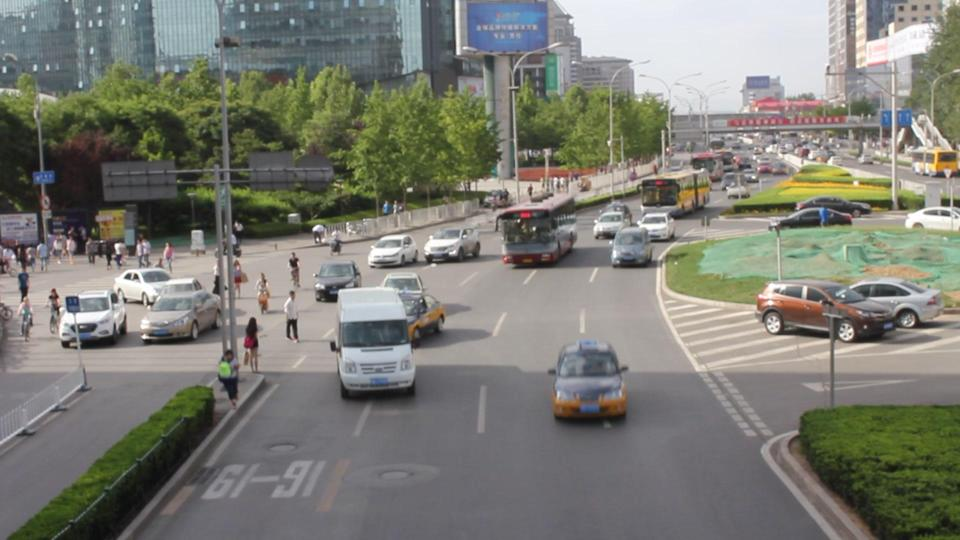
\includegraphics[scale=0.35]{gambar/Mobil2.jpg}
  % Keterangan gambar yang diinputkan
  \caption{Tangkapan Mobil dari Kamera Lalu Lintas}
  % Label referensi dari gambar yang diinputkan
  \label{fig:tangkapanmobildarikameralalulintas}
\end{figure}

Mobil (\emph{automobile}, \emph{motorcar}, atau \emph{car}) merupakan kendaraan yang umumnya beroda empat dan dirancang untuk bergerak 
menggunakan mesin pembakaran internal menggunakan bahan bakar yang mudah menguap. Mobil memiliki sistem teknis yang 
kompleks yang terdiri dari berbagai macam subsistem yang memiliki fungsinya masing-masing. Mobil telah menjadi sarana 
utama transportasi keluarga selama bertahun-tahun, dengan perkiraan 1,4 miliar mobil beroperasi di seluruh dunia. Desain 
dari mobil Sebagian besar bergantung dari tujuan penggunaannya. Seperti misalnya mobil dengan kegunaan \emph{off-road} harus tahan 
lama terhadap kondisi medan, sistemnya sederhana namun memiliki daya tahan tinggi terhadap beban berlebih. Sementara mobil 
yang digunakan di jalan raya dengan sistem kecepatan tinggi harus memiliki kondisi seperti performa mesin yang tinggi, 
memberikan kenyamanan pada penumpang, dan mobil memiliki stabilitas yang optimal \parencite{Cromer2023}. Perbedaan 
berdasarkan fungsi dan perusahaan manufaktur membuat mobil-mobil yang ada di dunia ini memiliki ciri khasnya masing-masing 
dan dapat dibedakan satu sama lain.

\section{Citra}
\label{sec:citra}

Citra atau gambar merupakan representasi visual dari suatu objek, seperti manusia, barang, maupun pemandangan. Citra 
umumnya terbagi menjadi dua jenis, yaitu citra analog dan citra digital. Citra analog memiliki sifat kontinyu dan tidak 
dapat direpresentasikan dalam komputer sehingga tidak dapat diproses oleh komputer secara langsung \parencite{Tyagi2018}. 
Sementara citra digital merupakan sebuah larik (array) yang berisi nilai-nilai real, kompleks, dan berhingga (\emph{finite}) 
yang direpresentasikan dengan deretan bit tertentu. 

\begin{figure}[ht]
  \centering
  % Nama dari file gambar yang diinputkan
  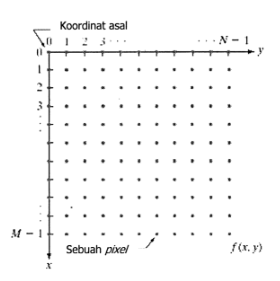
\includegraphics[scale=1]{gambar/Koordinat Citra Digital.png}
  % Keterangan gambar yang diinputkan
  \caption{Koordinat Citra Digital}
  % Label referensi dari gambar yang diinputkan
  \label{fig:koordinatcitradigital}
\end{figure}

Citra dapat didefinisikan sebagai fungsi f(x,y) berukuran M baris dan N kolom. x dan y pada fungsi merupakan koordinat 
spasial dan amplitude f di titik (x,y) adalah intensitas atau tingkat keabuan dari citra tersebut. Gambar 2.2 merupakan 
contoh sebuah koordinat citra digital \parencite{Putra2010}.

\section{\emph{Machine Learning}}
\label{sec:machinelearning}

\begin{figure}[ht]
  \centering
  % Nama dari file gambar yang diinputkan
  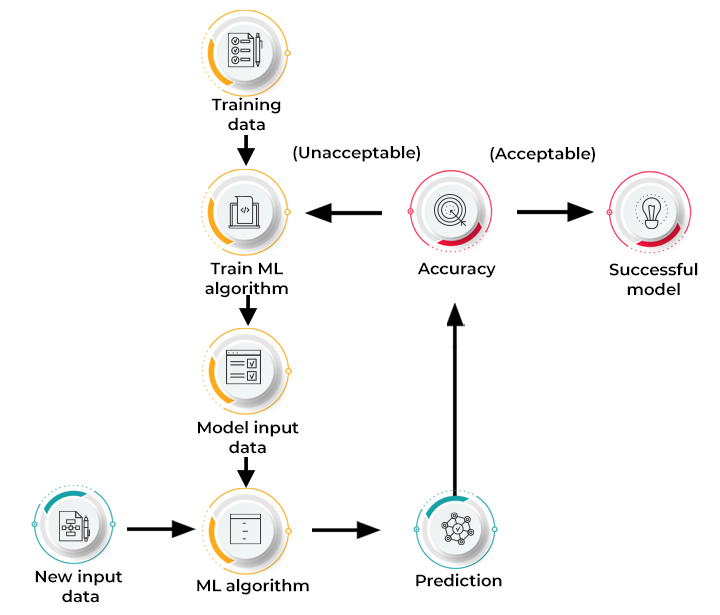
\includegraphics[scale=0.5]{gambar/How Machine learning work.png}
  % Keterangan gambar yang diinputkan
  \caption{Cara Kerja \emph{Machine Learning}}
  % Label referensi dari gambar yang diinputkan
  \label{fig:carakerjamachinelearning}
\end{figure}

\emph{Machine learning} (ML) merupakan salah satu disiplin dari \emph{Artificial Intelligence} (AI) dimana sebuah sistem akan 
mempelajari dan menganalisa data-data terdahulu secara otomatis. Sistem tersebut nantinya akan berfokus mengindetifikasi 
pola dari data yang telah didapat, mempelajari pola tersebut secara iteratif, kemudian membangun model berdasarkan data 
yang telah dipelajari, dan menggunakan model tersebut untuk membuat prediksi ketika diberikan sebuah data baru \parencite{Russel2021}.

Terdapat dua alasan utama perlunya membuat sebuah mesin yang dapat belajar. Alasan pertama karena pembuat mesin 
(machine designer) tidak dapat mengantisipasi seluruh kemungkinan yang ada di masa depan. Seperti misalnya sebuah robot 
yang didesain untuk menavigasikan sebuah labirin. Robot tersebut perlu mempelajari labirin tersebut sebelum dapat menavigasikannya. 
Alasan kedua yaitu karena adakalanya pembuat mesin justru tidak tahu bagaimana membuat sebuah kode untuk memecahkan permasalahan, 
sehingga menggunakan algoritma dari \emph{machine learning} untuk memecahkan masalah \parencite{Russel2021}.

\subsection{\emph{Supervised Learning}}

\emph{Supervised Learning} merupakan algoritma \emph{machine learning} yang mempelajari kumpulan input-output yang telah dipasangkan. 
Output yang telah dipasangkan ini disebut dengan label. \emph{machine learning} akan menerima beberapa input data yang telah 
dipasangkan dengan output, kemudian mempelajarinya dengan cara membandingkan output yang diperoleh dengan output yang benar. Seperti 
contohnya ketika diberikan input citra bergambar bis, maka akan memberikan output bertuliskan “bis”. Dengan \emph{Supervised Learning}, 
maka model \emph{machine learning} dapat mengklasifikasi data baru berdasarkan data training yang pernah dipelajari \parencite{Russel2021}.

\subsection{\emph{Unsupervised Learning}}

\emph{Unsupervised Learning} merupakan algoritma \emph{machine learning} yang mempelajari pola dari data yang tidak memiliki label, 
sehingga model tidak mengetahui benar atau tidaknya output yang diberikan. Umumnya \emph{Unsupervised Learning} akan mengelompokan 
(clustering) output berdasarkan contoh-contoh yang memiliki kemiripan. Contoh dari \emph{Unsupervised Learning} yaitu Ketika memberikan 
input citra bergambar kucing, maka model akan memberikan output berbagai macam citra yang memiliki kemiripan atau berhubungan dengan 
kucing \parencite{Russel2021}.

\section{\emph{Deep Learning}}
\label{sec:deeplearning}

\emph{Deep Learning} merupakan salah satu cabang dari \emph{machine learning} (ML) dimana model yang dibuat untuk mendapatkan output 
mengikuti bentuk model neuron dari otak manusia, sehingga sering juga disebut dengan \emph{neural network}. Metode \emph{Deep Learning} 
memiliki bentuk rangkaian yang memiliki banyak layer di dalamnya, sehingga data yang masuk akan melalui sejumlah layer yang telah ditetapkan 
hingga menjadi sebuah output. Tidak seperti metode lainnya yang dapat menangani banyak data dan memiliki waktu proses yang singkat, proses 
menggunakan metode \emph{Deep Learning} bergantung dari jumlah layer yang digunakan di dalam model. Semakin banyak layer yang digunakan mengakibatkan 
waktu untuk memproses data lebih lama karena tingkat kompleksitas yang semakin tinggi. Metode \emph{Deep Learning} banyak diaplikasikan pada 
\emph{visual object recognition}, \emph{machine translation}, \emph{speech recognition}, \emph{speech synthesis}, dan \emph{image synthesis} 
\parencite{Russel2021}.

\emph{Deep Learning} terbukti memiliki keunggulan yang lebih dibandingkan menggunakan \linebreak metode lainnya, khususnya data yang memiliki dimensi 
tinggi seperti citra. Seperti misalnya pada metode linear dan metode linear regression, kedua metode tersebut dapat menangani variabel input 
yang cukup besar, namun ketika dilakukan perhitungan, waktu yang dibutuhkan cukup singkat, karena setiap variabel input yang berbeda hanya 
berhubungan secara independen dengan output. Setiap variabel input ini tidak memiliki keterhubungan satu sama lain. Sifat dari metode ini 
menyebabkan model yang dihasilkan terbatasi kemampuannya. Model yang dihasilkan hanya sebatas mengikuti fungsi linear dan batas yang ada di 
bagian input. Dimana pada dunia nyata, konsep dan input yang harus diolah lebih kompleks. Hal inilah yang membuat \emph{Deep Learning} memiliki 
keunggulan yang signifikan. Gambar 2.4 merupakan contoh perbandingan dari jaringan komputasi yang dimiliki oleh metode \emph{linear regression}, metode 
\emph{decision list network}, dan metode \emph{deep learning} \parencite{Russel2021}. 

\begin{figure}[ht]
  \centering
  % Nama dari file gambar yang diinputkan
  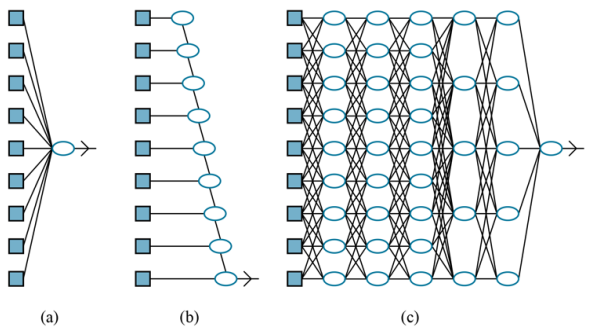
\includegraphics[scale=0.7]{gambar/Jaringan Deep learning.png}
  % Keterangan gambar yang diinputkan
  \caption{Perbedaan (a) \emph{Linear Regression}, (b) \emph{Decision List Network}, dan (c) \emph{Deep Learning}}
  % Label referensi dari gambar yang diinputkan
  \label{fig:perbedaanlinearregressiondecissionlistnetworkdeeplearning}
\end{figure}

\section{\emph{Re-identifikasi}}
\label{sec:re-identifikasi}

\begin{figure}[ht]
  \centering
  % Nama dari file gambar yang diinputkan
  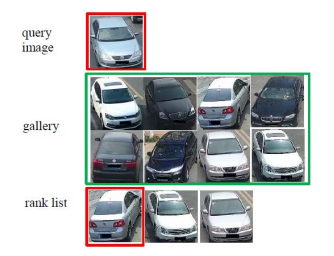
\includegraphics[scale=1]{gambar/Contoh Re-identification.png}
  % Keterangan gambar yang diinputkan
  \caption{Contoh Re-identifikasi}
  % Label referensi dari gambar yang diinputkan
  \label{fig:contohreidentifikasi}
\end{figure}

Re-identifikasi merupakan teknik mencocokan dua objek dengan bidang pandang berbeda berdasarkan kemiripan pada beberapa parameter yang telah 
ditentukan dengan tujuan untuk membuktikan bahwa kedua objek tersebut sama. Karakteristik dari re-identifikasi berupa sebuah siklus hipotesis-deduktif, 
dimana model prediksi yang dibuat dengan mempelajari training data akan mengumpulkan data baru dari masukan, kemudian diikuti dengan revisi dan 
pelabelan baru untuk data yang memiliki nilai kecocokan tinggi. Hal tersebut akan terus berulang mengikuti data terbaru yang dimasukan ke model 
prediksi tersebut \parencite{Wechsler2014}. Cara kerja model re-identifikasi dapat dilihat pada gambar 2.5. Pengguna akan memasukkan sebuah gambar 
kueri ke dalam model re-identifikasi. Model akan mencari gambar dengan objek yang memiliki kemiripan dengan gambar kueri di galeri. Gambar yang memiliki 
kemiripan dengan kueri kemudian akan dibuat list tingkat kemiripan gambar galeri berdasarkan gambar kueri.

Kebutuhan akan adanya sebuah sistem re-identifikasi dikaitkan dengan beberapa alasan, seperti untuk meningkatkan keamanan di lingkungan publik 
yang menyebabkan penyebaran kamera CCTV yang meluas di area seperti taman, kampus, sekolah, jalan raya, dan lainnya. Semakin banyaknya kamera CCTV 
di lingkungan publik berbanding lurus dengan semakin banyaknya tenaga kerja kasar manusia yang dibutuhkan untuk melihat dan melacak orang/kendaraan 
secara akurat dan efisien melalui kamera \parencite{Zheng2016}. Semakin sulitnya melakukan re-identifikasi secara manual menjadi alasan kuat perlu dikembangkannya 
sistem re-identifikasi yang akurat dan efisien.

\section{Transformer}
\label{sec:transformer}

Model transduksi urutan dominan (\emph{dominant sequence transduction model}) yang ada diciptakan menggunakan arsitektur \emph{convolutional neural network} 
(CNN) atau \emph{recurrent neural network} (RNN) kompleks, yang memiliki encoder dan decoder. Namun pada 2017, diperkenalkan arsitektur jaringan yang cukup 
simpel, yang disebut The Transformer. Arsitektur Transformer memperkenalkan sebuah sistem jaringan saraf yang berfokus pada mekanisme perhatian (\emph{attention}) 
dengan bantuan encoder dan decoder, tanpa menggunakan \emph{reccurent network} dan konvolusi seperti yang ada pada model \emph{sequence to sequence}. \parencite{Vaswani2017}

Ketika diperkenalkan,Transformer diuji cobakan untuk menjadi sebuah model penerjemah Bahasa. Ketika dibandingkan dengan model ber-asitektur CNN dan RNN 
(seperti Extended Neural GPU, ByteNet, dan ConvS2S), terbukti bahwa Transformer, sebuah arsitektur tanpa RNN dan hanya menggunakan mekanisme perhatian, dapat 
melakukan training lebih cepat dengan training data yang terbatas dan ukuran yang besar, serta skor output training yang dihasilkan pun juga mengungguli model-model 
ber-asitektur CNN dan RNN. \parencite{Vaswani2017}

\section{Swin Transformer}
\label{sec:swintransformer}

Pemodelan pada visi komputer telah lama didominasi oleh \emph{Convolutional Neural Network} (CNN), dimulai dengan AlexNet dan kinerja revolusinya di tantangan 
klasifikasi gambar ImageNet. Arsitektur CNN telah berevolusi menjadi arsitektur yang hebat dengan skala yang lebih besar, koneksi yang lebih luas, dan bentuk 
konvolusinya yang lebih canggih. Sementara arsitektur Transformer yang saat ini lazim digunakan pada \emph{Natural Language Processing} (NLP), justru tidak cocok 
ketika digunakan sebagai model pada visi komputer. Hal ini dikarenakan pada tugas visi komputer seperti segmentasi semantik, dibutuhkan fitur prediksi hingga pada 
tingkat piksel. Hal ini cukup sulit untuk arsitektur Transformer ketika dihadapkan gambar beresolusi tinggi, karena mekanisme kompleksitas komputasi \emph{self-attention} 
yang dimiliki bersifat kuadratik terhadap ukuran gambar. Sehingga untuk mengatasi masalah tersebut, diciptakanlah Swin Transformer. \parencite{Liu2021}

\begin{figure}[ht]
  \centering
  % Nama dari file gambar yang diinputkan
  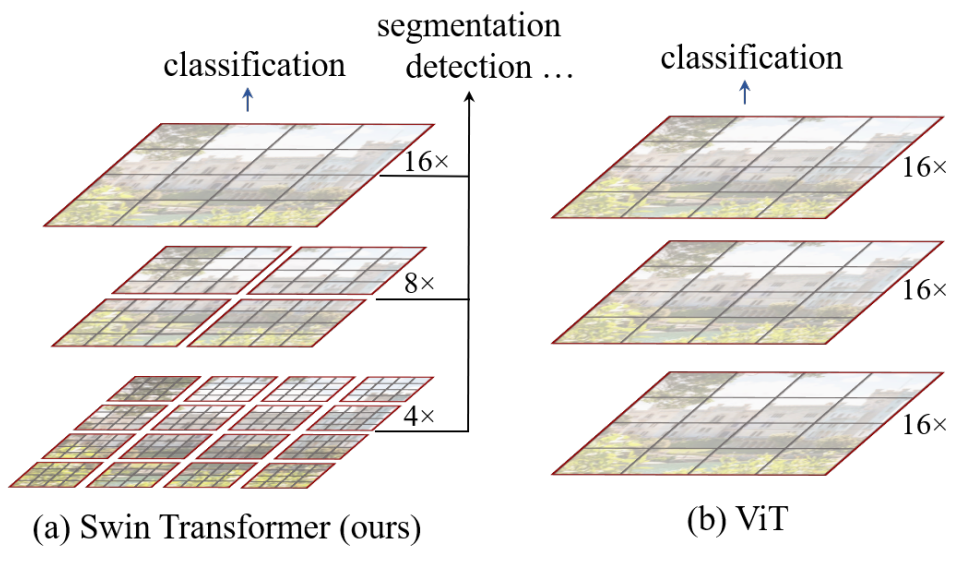
\includegraphics[scale=0.5]{gambar/Perbedaan Swin dan VIT.png}
  % Keterangan gambar yang diinputkan
  \caption{Perbedaan (a)  Swin Transformer dan (b) Vision Transformer}
  % Label referensi dari gambar yang diinputkan
  \label{fig:perbedaanswintransformerdanvisiontransformer}
\end{figure}

Swin Transformer sebagai sebuah arsitektur baru untuk visi komputer, mampu \linebreak memetakan hirarki dan kompleksitas komputasinya mengikuti ukuran gambar. Seperti yang 
terlihat pada gambar 2.6, Swin Transformer membangun sebuah hirarkis dengan \emph{patch} berukuran kecil (bergaris abu-abu) pada lapisan atas, yang kemudian secara 
bertahap \emph{patch} tersebut akan bergabung dengan sekitarnya di lapisan yang lebih dalam. Selain itu, Swin Transformer memiliki kompleksitas komputasi yang linear 
terhadap ukuran gambar dikarenakan komputasi \emph{self-attention} hanya berfokus pada setiap jendela (bergaris merah). Berbeda dengan Vision Transformer yang 
memetakan dengan resolusi rendah dan memiliki kompleksitas komputasi kuadratik terhadap ukuran gambar karena komputasi \emph{self-attention} dilakukan secara 
menyeluruh. \parencite{Liu2021}

\subsection{\emph{Shifted Windows}}

Arsitektur standar Transformer dan adaptasinya untuk klasifikasi gambar menggunakan \emph{global self-attention}. \emph{global self-attention} merupakan hubungan antara 
satu token dengan token lainnya ketika dikomputasikan. Perhitungan global ke kompleksitas kuadrat berhubungan dengan jumlah token. Hal ini membuat Transformer tidak cocok 
untuk menyelesaikan permasalahan visi yang membutuhkan kumpulan token yang besar untuk prediksi padat pada gambar beresolusi tinggi. \parencite{Liu2021}

\begin{figure}[ht]
  \centering
  % Nama dari file gambar yang diinputkan
  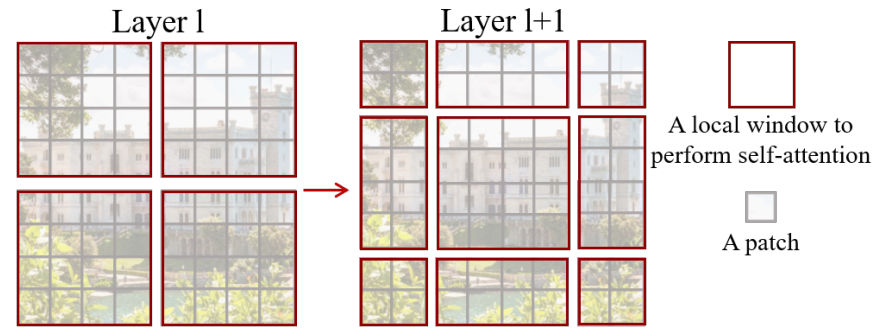
\includegraphics[scale=0.7]{gambar/Ilustrasi Shifted Windows.png}
  % Keterangan gambar yang diinputkan
  \caption{Ilustrasi Shifted-Windows}
  % Label referensi dari gambar yang diinputkan
  \label{fig:ilustrasishiftedwindows}
\end{figure}

Karenanya, diciptakanlah \emph{shifted windows} untuk memperbaiki kekurangan dari \linebreak transformer. Gambar 2.7 merupakan sebuah ilustrasi dari pendekatan \emph{shifted windows} 
untuk menghitung \emph{self-attention} yang dikenalkan pada arsitektur Swin Transformer. Pada layer 1 (kiri), skema partisi dari jendela biasa diadopsi, dan \emph{self-attention} 
akan dihitung pada setiap jendelanya. Kemudian pada layer \begin{math}1+1\end{math} (kanan), jendela partisi akan bergeser (\emph{shifted}) dan menghasilkan jendela baru. Perhitungan 
\emph{self-attention} di jendela yang baru melintasi Batasan dari jendela sebelumnya di layer 1, dimana menyediakan koneksi diantaranya. \parencite{Liu2021}

\subsection{Arsitektur Swin Transformer}

\begin{figure}[ht]
  \centering
  % Nama dari file gambar yang diinputkan
  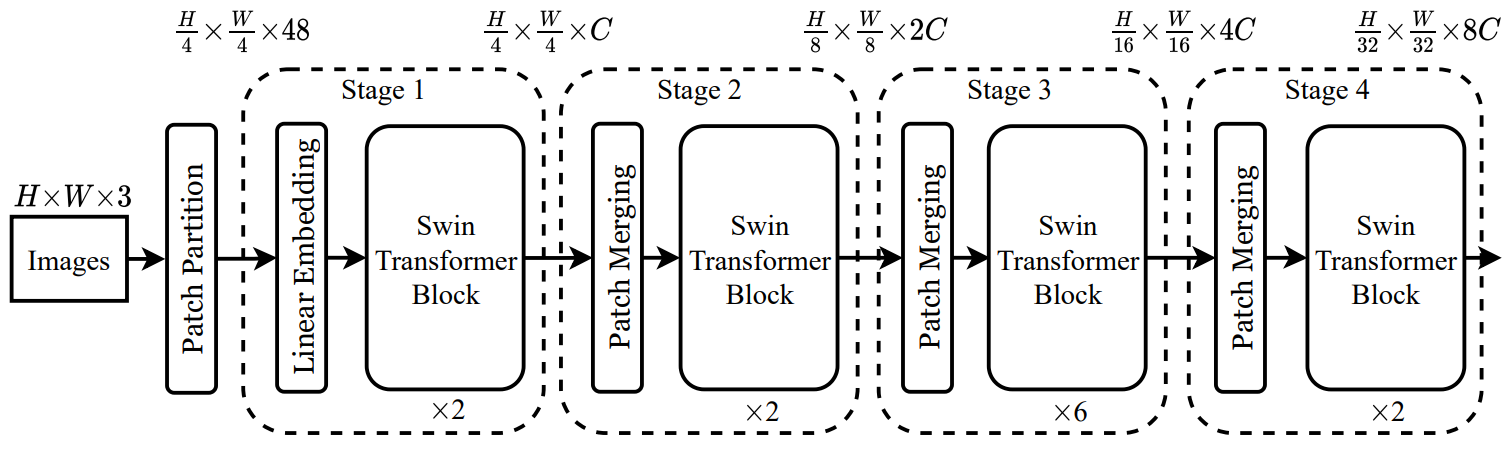
\includegraphics[scale=0.5]{gambar/Arsitektur Swin.png}
  % Keterangan gambar yang diinputkan
  \caption{Arsitektur Swin Transformer}
  % Label referensi dari gambar yang diinputkan
  \label{fig:arsitekturswintransformer}
\end{figure}

Gambaran dari arsitektur Swin Transformer dapat dilihat pada gambar 2.8, yang mengilustrasikan versi kecil dari Swin Transformer (Swin-T). Pada tahap awal, gambar input akan 
dibagi menjadi \emph{patch} non-tumpang tindih menggunakan modul pemecah tambalan, seperti ViT. Setiap \emph{patch} yang dihasilkan diperlakukan sebagai “token” dan fiturnya ditetapkan sebagai 
rangkaian dari nilai RGB piksel mentah. Dalam implementasinya, ukuran \emph{patch} yang digunakan adalah \begin{math}4 \times 4\end{math}, sehingga dimensi fitur dari masing-masing \emph{patch} adalah 
\begin{math}4 \times 4 \times 3 = 48\end{math}. Lapisan linear diterapkan pada fitur bernilai mentah ini untuk memproyeksikannya ke sembarang dimensi (dilambangkan sebagai C). \parencite{Liu2021}

Beberapa blok Transformer dengan perhitungan \emph{self-attention} yang dimodifikasi diterapkan pada token \emph{patch} ini. Blok Transformer mempertahankan jumlah tokennya 
(\begin{math}\frac{H}{4} \times \frac{H}{4}\end{math}), dan bersama dengan penyematan linear disebut dengan “tahap 1”. \parencite{Liu2021}

Untuk menghasilkan representasi hierarkis, semakin dalamnya jaringan akan membuat jumlah token dikurangi dengan lapisan yang menggabungkan \emph{patch}. Lapisan penggabungan \emph{patch} pertama menggabungkan 
fitur dari setiap kelompok \emph{patch} sekitarnya \begin{math}2 \times 2\end{math}, yang kemudian diterapkan di lapisan linear pada rangkaian fitur dimensi 4C. Hal ini mengurangi jumlah token dengan 
kelipatan \begin{math}2 \times 2 = 4\end{math} (\begin{math}2 \times resolusi downsampling\end{math}), dan dimensi keluarannya diatur ke 2C. Blok Swin Transformer diterapkan setelahnya untuk 
transformasi fitur, dengan resolusi tetap pada \begin{math}\frac{H}{8} \times \frac{W}{8}\end{math}. Blok penggabungan patch pertama yang ditambah dengan transformasi fitur dinotasikan sebagai 
“tahap 2”. Kemudian prosedur ini diulang dua kali, sebagai “tahap 3” dan “tahap 4”, dengan resolusi keluaran dari \begin{math}\frac{H}{16} \times \frac{W}{16}\end{math} dan 
\begin{math}\frac{H}{32} \times \frac{W}{32}\end{math}. Tahapan-tahapan ini menghasilkan representasi hierarkis, dengan resolusi peta fitur yang sama dengan jaringan konvolusional. \parencite{Liu2021}

\subsection{Blok Swin Transformer}

\begin{figure}[ht]
  \centering
  % Nama dari file gambar yang diinputkan
  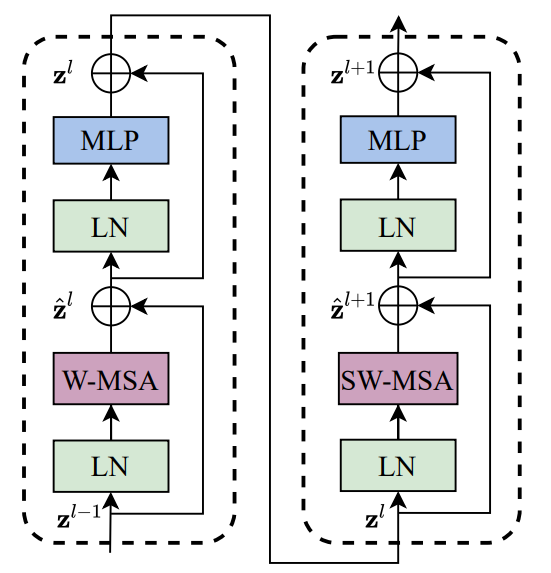
\includegraphics[scale=0.6]{gambar/Blok Swin.png}
  % Keterangan gambar yang diinputkan
  \caption{Blok Swin Transformer}
  % Label referensi dari gambar yang diinputkan
  \label{fig:blokswintransformer}
\end{figure}

Swin Transformer dibangun dengan menggantikan standar modul \emph{multi-head self attention} (MSA) di dalam blok Transformer dengan modul \emph{shifted windows} (dijelaskan pada bagian 2.8.1), dengan 
lapisan lain tetap sama. Seperti yang diilustrasikan pada gambar 2.9, blok Swin Transformer terdiri dari \emph{shifted windows} dengan basis modul MSA, yang kemudian diikuti 2 layer MLP dengan 
nonlinear GELU diantaranya. Lapisan \emph{LayerNorm} (LN) diterapkan sebelum setiap modul MSA dan MLP, dan residu koneksi diterapkan di setiap setelah modul. \parencite{Liu2021}

\subsection{Variasi Model}

Swin Transformer memiliki beberapa variasi model yang dapat digunakan. Swin-B (\emph{Swin Base}) dibuat dengan ukuran model dan tingkat kompleksitas komputasi yang mirip dengan ViT-B 
(\emph{Vision Transformer Base}). Selain itu, dikenalkan juga varian model Swin-T, Swin-S, dan Swin-L. Swin-T (\emph{Swin Tiny}) merupakan versi 0.25x ukuran dan tingkat kompleksitas 
komputasi dari \emph{base}. Swin-S (\emph{Swin Small}) merupakan versi 0.5x dari \emph{base}, sementara Swin-L (\emph{Swin Large}) merupakan versi 2x dari \emph{base}. Swin-T dan Swin-S 
memiliki kompleksitas yang mirip dengan ResNet-50 dan ResNet-101. Ukuran jendela diatur ke M = 7 secara default. Sementara dimensi kueri pada setiap kepala adalah d = 32, dan lapisan 
ekspansi di setiap MLP adalah \begin{math}\alpha = 4\end{math}, untuk semua parameter. Hyper-parameter dari setiap variasi modelnya adalah sebagai berikut:

\begin{itemize}[nolistsep]

  \item Swin-T: C = 96, Jumlah layer = \verb|{2,2,6,2}|

  \item Swin-S: C = 96, Jumlah layer = \verb|{2,2,18,2}|

  \item Swin-B: C = 128, Jumlah layer = \verb|{2,2,18,2}|

  \item Swin-L: C = 192, Jumlah layer = \verb|{2,2,18,2}|

\end{itemize}

C merupakan nomor saluran dari lapisan tersembunyi di tahap pertama.\parencite{Liu2021}

Setelah dilakukan percobaan di 3 jenis tugas, hasil percobaan menunjukan bahwa Swin Transformer memiliki performa yang bagus untuk digunakan di tugas visi. Hal ini dikarenakan pada klasifikasi gambar, Swin 
Transformer mendapatkan akurasi 84,5 pada ImageNet-1K dan akurasi 87,3 pada ImageNet-22K pre-trained models. Kemudian pada deteksi objek, Swin Transformer mendapatkan nilai 58,7 untuk box AP dan 51,1 
untuk mask AP pada pengembangan deteksi objek COCO. Dan pada segmentasi semantik, Swin Transformer mendapatkan nilai 53.5 untuk mIoU pada ADE20K. Hal ini menunjukan bahwa Swin Transformer memiliki potensi 
untuk menjadi basis di tugas visi.\parencite{Liu2021}

\section{Swin Transformer V2}
\label{sec:swintransformerv2}

Swin Transformer merupakan salah satu \emph{backbone} dalam tugas umum di visi computer yang memiliki performa kuat di berbagai tugas pengenalan granular, seperti \emph{region-level object detection}, 
\emph{pixel-level semantic segmentation}, dan klasifikasi citra. Gagasan utama dari Swin Transformer adalah untuk mengenalkan beberapa prior visual penting ke dalam encoder Transformer, termasuk hirarki, 
lokalitas, dan invarian terjemahan. Dengan pengenalan ini membuat backbone memiliki dua kekuatan yang digabungkan, yaitu unit Transformer dasar yang memiliki kemampuan pemodelan yang kuat, dan prior 
visual yang ramah terhadap berbagai tugas visual.\parencite{Liuv22021}

\begin{figure}[ht]
  \centering
  % Nama dari file gambar yang diinputkan
  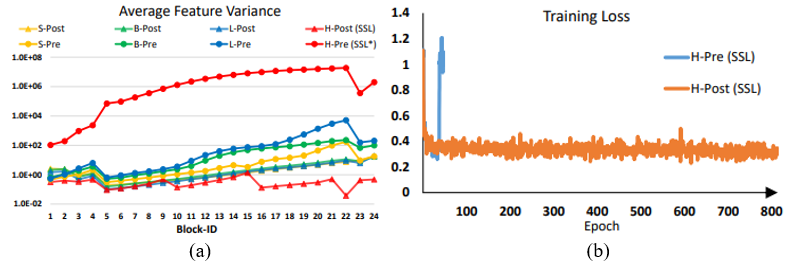
\includegraphics[scale=0.9]{gambar/Issue Swin V1.png}
  % Keterangan gambar yang diinputkan
  \caption{(a)Plotingan Sinyal propogasi, (b)Hasil Training Model \emph{Huge}}
  % Label referensi dari gambar yang diinputkan
  \label{fig:plotingansinyalpropogasidanperbedaanhasiltrainingmodelhuge}
\end{figure}

Namun ketika dilakukan peningkatan kapasitas dan resolusi jendela dari Swin \linebreak Transformer, ditemukan dua masalah. Ketika kapasitas dari model Swin Transformer ditingkatkan, terdapat masalah ketidakstabilan 
pada plotingan sinyal propogasi seperti yang terlihat di gambar 2.10(a). Ketika model Swin Transformer diperbesar dari ukuran \emph{small} (Swin-S) ke ukuran \emph{large} (Swin-L), nilai aktivasi di lapisan 
yang lebih dalam meningkat secara dramatis. Perbedaan antar lapisan dengan amplitudo tertinggi dan terendah mencapai nilai ekstrim sebesar 104. Ketika model Swin Transformer diperbesar hingga ukuran 
\emph{Huge} (Swin-H), model tidak dapat menyelesaikan training seperti pada gambar 2.10(b).\parencite{Liuv22021}

\begin{figure}[ht]
  \centering
  % Nama dari file gambar yang diinputkan
  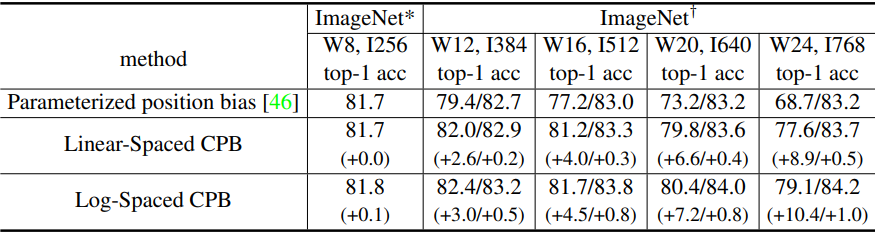
\includegraphics[scale=0.75]{gambar/Penurunan kinerja Swin v1.png}
  % Keterangan gambar yang diinputkan
  \caption{Perbandingan Hasil Berbagai Pendekatan Perhitungan Bias Posisi}
  % Label referensi dari gambar yang diinputkan
  \label{fig:perbandinganberbagaihasilpendekatanperhitunganbiasposisi}
\end{figure}

Masalah kedua yaitu adanya penurunan kinerja saat mentransfer model di seluruh resolusi jendela. Seperti yang terlihat pada gambar 2.11 pada baris pertama (\emph{Parameter position bias}), akurasi menurun secara 
signifikan ketika dilakukan pengujian akurasi model \emph{pre-trained} Image-Net-1K (dengan gambar \begin{math}256\times256\end{math} dan ukuran jendela \begin{math}8\times8\end{math}) pada resolusi gambar dan ukuran 
jendela yang lebih besar melalui pendekatan interpolasi bi-kubik. Sehingga perlu adanya pemeriksaan terkait pendekatan bias posisi relatif di Swin Transformer. Pemecahan kedua masalah ini adalah dengan perubahan 
pada sisi arsitektur Swin Transformer, dan revisi dari Swin Transformer ini disebut dengan Swin Transformer V2.\parencite{Liuv22021}

\subsection{Arsitektur Swin Transformer V2}

\begin{figure}[ht]
  \centering
  % Nama dari file gambar yang diinputkan
  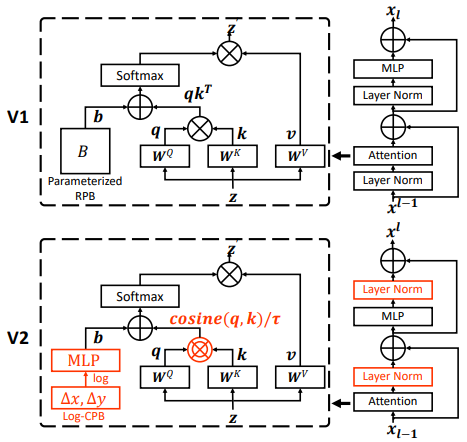
\includegraphics[scale=0.75]{gambar/Perbedaan V1 V2.png}
  % Keterangan gambar yang diinputkan
  \caption{Perbedaan Arsitektur Swin Transformer V1 dan V2}
  % Label referensi dari gambar yang diinputkan
  \label{fig:perbandinganarsitekturswintransformerv1danv2}
\end{figure}

Perubahan arsitektur Swin Transformer V1 ke V2 dapat dilihat pada gambar 2.12. Terdapat tiga bagian dari arsitektur Swin Transformer yang diadaptasi, yaitu \emph{res-post-norm} menggantikan konfigurasi 
\emph{pre-norm} sebelumnya, penambahan kosinus berskala untuk menggantikan \emph{dot product} pada bagian \emph{attention}, dan pergantian pendekatan parameterisasi pada V1 menjadi pendekatan bias posisi 
relatif kontinu dengan \emph{log-spaced}.\parencite{Liuv22021}

Adaptasi \emph{res-post-norm} dan penambahan kosinus berskala memudahkan model untuk \linebreak meningkatkan kapasitas. Sementara pergantian pendekatan bias posisi relatif kontinu membuat model ditransfer lebih 
efektif melewati resolusi jendela.\parencite{Liuv22021}

\subsection{Variasi Model Swin Transformer V2}

Swin Transformer V2 tetap mempertahankan pengaturan tahap, jumlah layer, dan saluran untuk 4 konfigurasi dari Swin Transformer V1, yaitu:

\begin{itemize}[nolistsep]

  \item SwinV2-T: C = \verb|96,#|. Jumlah layer = \verb|{2,2,6,2}|

  \item SwinV2-S/B/L: C = \verb|96/128/192,#|. Jumlah layer = \verb|{2,2,18,2}|

\end{itemize}

Dengan C merupakan nomor saluran di tahap pertama.

Kemudian Swin Transformer V2 juga meningkatkan skalanya ke tingkat \emph{huge} (SwinV2-H) dan tingkat \emph{giant} (SwinV2-G). SwinV2-H memiliki jumlah parameter sebanyak 658 juta, sementara SwinV2-G memiliki 
jumlah parameter 3 miliar parameter. Nomor saluran dan jumlah layer untuk masing-masingnya yaitu:

\begin{itemize}[nolistsep]

  \item SwinV2-H: C = \verb|352,#|. Jumlah layer = \verb|{2,2,18,2}|

  \item SwinV2-S/B/L: C = \verb|512,#|. Jumlah layer = \verb|{2,2,42,2}|

\end{itemize}

Terdapat penambahan lapisan normalisasi pada cabang utama di setiap 6 lapisan khusus untuk model SwinV2-H dan SwinV2-G. Karena alasan penghematan waktu eksperimen, \linebreak SwinV2-G hanya digunakan untuk eksperimen 
berskala besar, sementara SwinV2-H untuk studi paralel lain mengenai \emph{self-supervised learning}.\parencite{Liuv22021}

\section{VRIC Dataset}
\label{sec:vricdataset}

Selama dua tahun terakhir, re-identifikasi kendaraan menjadi perhatian dikarenakan \linebreak memiliki potensi untuk lebih fleksibel dalam melakukan pengenalan dan pencarian kendaraan dibandingkan 
menggunakan \emph{Automatic Number Plate Recognition} (ANPR). Walaupun begitu, re-identifikasi kendaraan berdasarkan penampilan visual menjadi tantangan tersendiri dikarenakan kemungkinan 
kendaraan memiliki penampilan yang sangat mirip dimana kendaraan yang berbeda namun jenis dan warna, model yang sama serta visual model yang bervariasi \linebreak berdasarkan posisi pengambilan 
gambar. Studi re-identifikasi kendaraan yang ada umumnya menggunakan salah satu dari dua dataset ini, yaitu VehicleID dan VeRi-776. Walaupun hasil studi menunjukkan hasil cukup memuaskan, 
namun pengaplikasian di dunia nyata belum jelas, dikarenakan dataset yang digunakan menggunakan gambar berkualitas tinggi dengan resolusi tinggi, tidak ada \emph{motion blur}, kondisi cuaca 
khusus, dan oklusi. Karena alasan inilah, diciptakan sebuah dataset baru yaitu \emph{Vehicle Re-Identification in Context} (VRIC). Perbedaan dataset antara VehicleID, VeRi-776, dan VRIC 
dapat dilihat pada gambar 2.13.\parencite{Kanaci2018}

\begin{figure}[ht]
  \centering
  % Nama dari file gambar yang diinputkan
  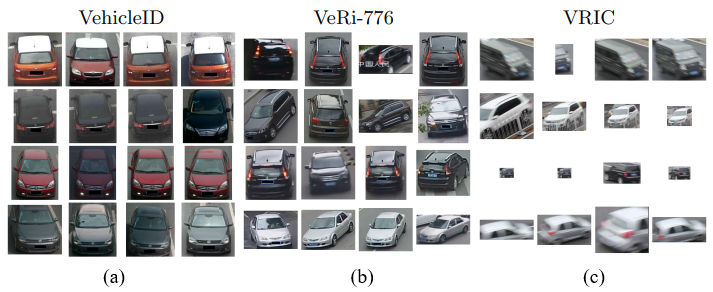
\includegraphics[scale=1]{gambar/Perbedaan VRIC dkk.png}
  % Keterangan gambar yang diinputkan
  \caption{Perbedaan (a)VehicleID, (b)VeRi-776, dan (c)VRIC}
  % Label referensi dari gambar yang diinputkan
  \label{fig:perbedaanvehicleidveri776danvric}
\end{figure}

VRIC merupakan dataset yang lebih realistis dan menantang yang dikhususkan untuk re-identifikasi kendaraan. VRIC berisikan 60.430 gambar dengan 5.622 ID kendaraan yang diambil dari 60 
kamera lalu lintas yang berbeda. VRIC berbeda dengan dataset dua dataset lainnya karena gambar yang diambil memiliki resolusi gambar yang bervariasi, terdapat \emph{motion blur}, kondisi 
cuaca yang bermacam-macam, dan oklusi. Hal ini membuat VRIC dapat memberikan benchmark dari re-identifikasi kendaraan yang lebih realistis. \parencite{Kanaci2018}

\subsection{Sumber Gambar}

Karena terdapat keterbatasan dalam pengaksesan data video pengawasan, sehingga VRIC menggunakan set data kendaraan yang tersedia untuk umum yang disediakan oleh komunitas riset. Sumber 
data kendaraan diambil dari UA-DETRAC \emph{object detection and tracking benchmark} dengan pertimbangan sebagai berikut:

\begin{itemize}[nolistsep]

  \item Seluruh video ditangkap dari adegan lalu lintas yang berada di dunia nyata, mencerminkan konteks “realistis” untuk re-identifikasi kendaraan.

  \item Video yang ada mencakup 24 lokasi penangkapan yang berbeda dengan kondisi lingkungan yang beragam, sehingga menawarkan skenario pengujian yang kaya tanpa bias terhadap kondisi 
  tertentu. 

  \item Berisi anotasi objek dan atribut yang kaya yang dapat memfasilitasi pelabelan ID untuk re-identifikasi kendaraan.

\end{itemize}

\begin{figure}[ht]
  \centering
  % Nama dari file gambar yang diinputkan
  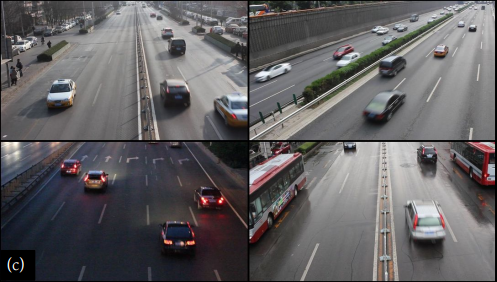
\includegraphics[scale=1]{gambar/Contoh lalu lintas VRIC.png}
  % Keterangan gambar yang diinputkan
  \caption{Contoh tangkapan gambar lalu lintas yang digunakan VRIC}
  % Label referensi dari gambar yang diinputkan
  \label{fig:contohtangkapangambarlalulintasyangdigunakanvric}
\end{figure}

Contoh tangkapan gambar lalu lintas dapat dilihat pada gambar 2.14.\parencite{Kanaci2018}

\subsection{Filter dan Anotasi Gambar}

\begin{figure}[ht]
  \centering
  % Nama dari file gambar yang diinputkan
  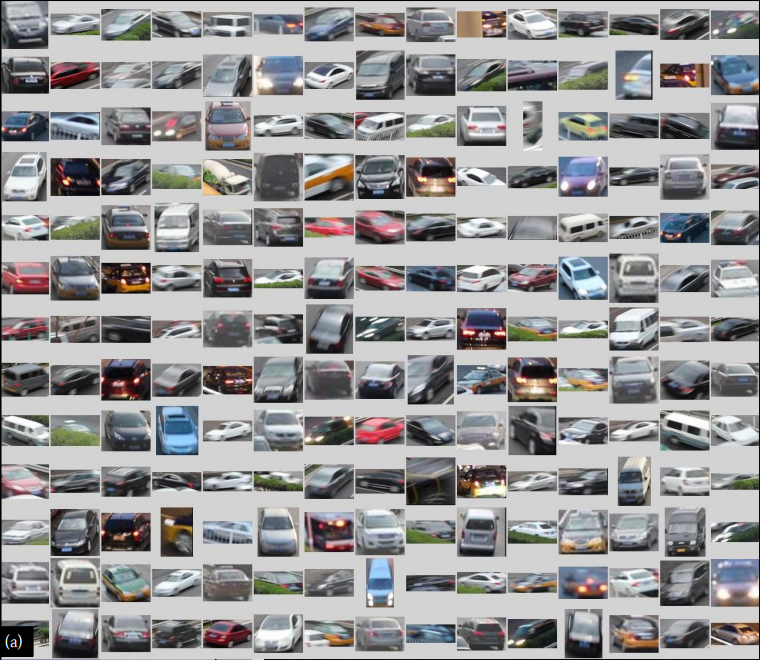
\includegraphics[scale=0.7]{gambar/Contoh boundingbox VRIC.png}
  % Keterangan gambar yang diinputkan
  \caption{Contoh Gambar dari Dataset VRIC}
  % Label referensi dari gambar yang diinputkan
  \label{fig:contohgambardaridatasetvric}
\end{figure}

Dataset VRIC dibuat dengan menggunakan 60 training video dengan anotasi objek \emph{bounding-box} yang berasal dari UA-DETRAC. Anotasi identitas kendaraan (ID) dilakukan dengan menetapkan 
label unik untuk setiap lintasan kendaraan per video UA-DETRAC, kemudian memverifikasi duplikasi ID secara manual. Dikarenakan seluruh video mentah UA-DETRAC diambil dari waktu dan adegan 
yang berbeda, ditemukan sedikit lintasan duplikat dalam hal identitas. Untuk membuat cukup banyak variasi tampilan kendaraan, maka dibuanglah lintasan pendek yang memiliki kurang dari 20 
frame, dan \emph{bounding-box} yang lebih kecil dari \begin{math}24 \times 24\end{math}. Sehingga dengan dilakukannya hal tersebut, didapatkan 5.622 ID kendaraan dari keseluruhan 60 video. 
\parencite{Kanaci2018}

Seperti yang terlihat di gambar 2.15, rata-rata resolusi gambar dari 60.430 \emph{bounding-box} kendaraan adalah \begin{math}69,8 \times 107,5\end{math} piksel pada 
\begin{math}lebar \times tinggi\end{math}, dengan variasi 32 hingga 280 piksel dikarenakan jarak yang tidak dibatasi antara kendaraan dan kamera. \parencite{Kanaci2018}

\subsection{Splitting Dataset}

\begin{figure}[ht]
  \centering
  % Nama dari file gambar yang diinputkan
  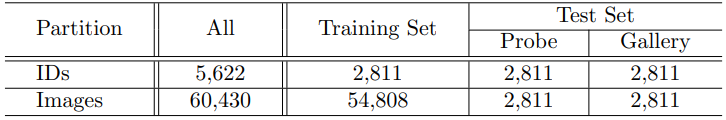
\includegraphics[scale=0.8]{gambar/Pembagian dataset VRIC.png}
  % Keterangan gambar yang diinputkan
  \caption{Pembagian Dataset VRIC}
  % Label referensi dari gambar yang diinputkan
  \label{fig:pembagiandatasetvric}
\end{figure}

Untuk model \emph{training} dan \emph{testing} menggunakan VRIC dataset sebagai benchmark, 5.622 ID kendaraan dari VRIC dibagi secara acak menjadi dua dan tidak tumpang tindih, dengan 
2.811 untuk \emph{training}, dan 2.811 untuk \emph{testing}. Karena tidak ada pencocokan ID berpasangan lintas kamera, maka disimulasikan variasi tampilan silang dengan pengambilan 
sampel jarak jauh antara gambar \emph{probe} dan \emph{gallery}. \parencite{Kanaci2018} Pembagian data untuk kebutuhan \emph{training} dan \emph{testing} dapat dilihat pada gambar 2.16.

\begin{figure}[ht]
  \centering
  % Nama dari file gambar yang diinputkan
  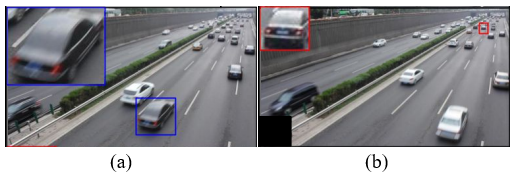
\includegraphics[scale=1]{gambar/Tampilan Dekat dan Jauh.png}
  % Keterangan gambar yang diinputkan
  \caption{Tampilan Semu (a)Dekat dan (b)Jauh dari VRIC}
  % Label referensi dari gambar yang diinputkan
  \label{fig:tampilansemuvric}
\end{figure}

Secara khusus, VRIC memiliki dua tampilan semu, yaitu dekat atau jauh, untuk setiap video dan kemudian akan dibangun set \emph{probe/gallery} dari lintasan uji dengan mengambil sampel 
dari dua tampilan semu tersebut secara acak. Tampilan jarak jauh dan dekat ini menghasilkan kondisi yang sangat berbeda dan memungkinkan untuk digunakan pada simulasi dari dua pandangan 
kamera yang tidak tumpang tindih. \parencite{Kanaci2018}


% % Contoh input gambar
% \begin{figure}[ht]
%   \centering

%   % Ubah dengan nama file gambar dan ukuran yang akan digunakan
%   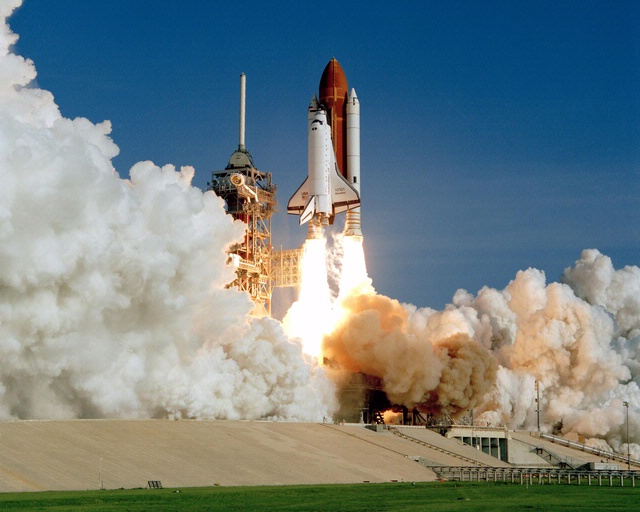
\includegraphics[scale=0.35]{gambar/roketluarangkasa.jpg}

%   % Ubah dengan keterangan gambar yang diinginkan
%   \caption{Peluncuran roket luar angkasa \emph{Discovery} \parencite{roketluarangkasa}.}
%   \label{fig:roketluarangkasa}
% \end{figure}

% Roket luar angkasa merupakan \lipsum[1]

% \emph{Discovery}, Gambar \ref{fig:roketluarangkasa}, merupakan \lipsum[2]

% \section{Gravitasi}
% \label{sec:gravitasi}

% Gravitasi merupakan \lipsum[1]

% \subsection{Hukum Newton}
% \label{subsec:hukumnewton}

% Newton \parencite{newton1687} pernah merumuskan bahwa \lipsum[1]
% Kemudian menjadi persamaan seperti pada persamaan \ref{eq:hukumpertamanewton}.

% % Contoh pembuatan persamaan
% \begin{equation}
%   \label{eq:hukumpertamanewton}
%   \sum \mathbf{F} = 0\; \Leftrightarrow\; \frac{\mathrm{d} \mathbf{v} }{\mathrm{d}t} = 0.
% \end{equation}

% \subsection{Anti Gravitasi}
% \label{subsec:antigravitasi}

% Anti gravitasi merupakan \lipsum[1]

\cleardoublepage

% Bab 3 desain dan implementasi
\chapter{METODOLOGI}
\label{chap:metodologi}

% Ubah bagian-bagian berikut dengan isi dari desain dan implementasi

% Penelitian ini dilaksanakan sesuai dengan batasan-batasan masalah yang telah disebutkan
% pada bagian 1.3. Berikut ini adalah beberapa peralatan dan perangkat yang terlibat dalam
% penelitian ini.

\section{Metode yang Digunakan}
\label{sec:metodeyangdigunakan}

Tugas akhir ini merupakan penelitian di bidang visi komputer dengan tujuan untuk melakukan 
re-identifikasi mobil menggunakan kumpulan citra dari dataset VRIC. Alur blok diagram metodologi 
dapat dilihat pada gambar 3.1. Perancangan model menggunakan metode Swin Transformer dari 
\emph{Pytorch ReID layumi}.

\begin{figure}[ht]
  \centering
  % Nama dari file gambar yang diinputkan
  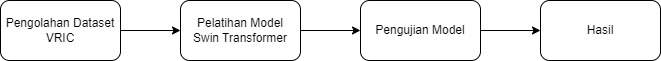
\includegraphics[scale=0.65]{gambar/metodologiFix.jpg}
  % Keterangan gambar yang diinputkan
  \caption{Diagram Blok Metodologi}
  % Label referensi dari gambar yang diinputkan
  \label{fig:diagramblokmetodologi}
\end{figure}

\begin{enumerate}[nolistsep]

  \item \textbf{Pengolahan Dataset VRIC}
  
  Pada tahapan ini, dilakukan proses pengolahan dataset yang didapat dengan 
  membagi dataset menjadi dua yaitu data training dan data test. Kedua data 
  ini nantinya akan digunakan untuk tujuan yang berbeda.

  \item \textbf{Pelatihan Model Swin Transformer}
  
  Pada tahapan ini, dilakukan training dan tuning pada model Swin Transformer 
  dengan mengubah parameternya. Parameter yang perlu disetel seperti 
  \emph{Loss Function}, \emph{Optimizer Function}, dan \emph{Epoch}.

  \item \textbf{Pengujian Model}
  
  Pada tahapan ini, model Swin Transformer yang telah melalui training dan 
  tuning akan diuji. Pengujian dilakukan menggunakan data test VRIC yang sebelumnya 
  telah dibagi.

  \item \textbf{Hasil}
  
  Jika hasil dari pengujian telah mencapai threshold dan model dapat melakukan \linebreak
  re-identifikasi dengan baik, maka seluruh hasil pengujian dicatat untuk dibandingkan 
  dengan penelitian yang sudah ada sebelumnya.

\end{enumerate}

\section{Bahan dan Peralatan yang Digunakan}
\label{sec:bahandanperalatanyangdigunakan}

\subsection{Dataset}

Dataset yang digunakan dalam penelitian ini adalah VRIC dataset. VRIC dataset memuat 
60 ribu citra mobil yang diambil dari kamera CCTV dari berbagai sudut pandang, sudut 
pencahayaan, dan kondisi lingkungan yang bermacam-macam. Setiap citra mobil dari VRIC 
dataset telah diberikan label sesuai dengan id vehicle dan id kamera yang mengambil 
citra tersebut.

%gambar 3.2 dataset

Gambar 3.2 merupakan beberapa contoh citra yang ada di VRIC dataset. Di dalam VRIC 
dataset, 60 ribu citra mobil telah dibagi ke tiga folder yang berbeda, yaitu folder 
\emph{train}, \emph{gallery}, dan \emph{query}. Folder \emph{train} berisikan 54 
ribu citra, sementara pada folder \emph{gallery} dan \emph{query} masing-masing 
berisikan 2 ribu citra. Terdapat pula list anotasi dari seluruh citra yang berisikan 
format nama file citra, label ID dari mobil, dan label kamera.

\subsection{Laptop}

Laptop digunakan untuk melakukan pemisahan (\emph{splitting}) dataset, training model, 
dan melakukan testing model yang telah selesai ditraining menggunakan VRIC dataset. 
Laptop perlu terhubung dengan internet untuk mengakses google Colaboratory, yang 
merupakan environment yang dibutuhkan untuk membuat model Swin Transformer. Spesifikasi 
laptop yang digunakan dapat dilihat pada tabel 3.1.

\begin{table}[ht]
  \begin{center}
  \caption{Spesifikasi Perangkat Laptop yang Digunakan}
  \label{tb:spesifikasilaptop}
  \begin{tabular}{|l|l|}
      \hline
      \textit{\textbf{Processor}}        & \begin{tabular}[c]{@{}l@{}}Intel Core i7-8750H \\ CPU @ 2.2 GHz\end{tabular} \\ \hline
      \textit{\textbf{Storage}}          & \begin{tabular}[c]{@{}l@{}}SSHD 1 TB Storage\\ SSD 128 GB Storage\end{tabular}         \\ \hline
      \textit{\textbf{RAM}}              & \begin{tabular}[c]{@{}l@{}}16 GB SODIMM DDR4 \\ 2666 MHz Dual Channel\end{tabular}    \\ \hline
      \textit{\textbf{Graphic Card}}     & \begin{tabular}[c]{@{}l@{}}NVIDIA GeForce GTX 1050 Ti \\ 4 GB GDDR5\end{tabular}      \\ \hline
      \textit{\textbf{Operating System}} & \begin{tabular}[c]{@{}l@{}}Windows 10 Home \\ Single Language 64-bit\end{tabular}     \\ \hline
  \end{tabular}
  \end{center}
\end{table}

\subsection{Google Colaboratory}

Google Colaboratory merupakan sebuah environment komputasi cloud dengan format \linebreak notebook 
yang disediakan oleh \emph{Google research} dengan fungsi untuk menjalankan kode python 
yang telah dituliskan. Google Colaboratory sangat membantu dalam pengerjaan \emph{data science}, 
\emph{deep learning}, dan \emph{machine learning} dikarenakan spesifikasi \emph{hardware} 
yang tinggi dari Google Colaboratory. Spesifikasi Google Colaboratory yang digunakan dapat 
dilihat pada tabel 3.2.

\begin{table}[ht]
  \begin{center}
  \caption{Spesifikasi Google Colaboratory}
  \label{tb:spesifikasigooglecolaboratory}
  \begin{tabular}{|l|l|}
      \hline
      \textit{\textbf{Processor}}        & \begin{tabular}[c]{@{}l@{}}Intel(R) Xeon(R) \\ CPU @ 2.2 GHz\end{tabular} \\ \hline
      \textit{\textbf{Graphic Card}}     & \begin{tabular}[c]{@{}l@{}}NVIDIA A100 SXM \\ 40 GB HBM2\end{tabular}      \\ \hline
  \end{tabular}
  \end{center}
\end{table}

\section{Urutan Pelaksanaan Penelitian}
\label{sec:urutanpelaksanaanpenelitian}

\subsection{Pemisahan Dataset}

VRIC dataset terbagi menjadi 3 bagian, yaitu data training, data query, dan data gallery. Ketiga 
bagian dataset tersebut telah dipisahkan dan disesuaikan secara langsung oleh developer dari VRIC 
dataset untuk kegunaan re-identifikasi mobil. Selain file berisi dataset, di dalam VRIC dataset 
juga terdapat file txt yang berisi list anotasi dari seluruh citra, dengan format nama file citra, 
label ID dari mobil, dan label kamera. Dengan menggunakan list anotasi tersebut, maka setiap dataset 
perlu dilakukan perubahan nama file sesuai dengan label ID dan label kameranya.

% Potongan kode rename
\lstinputlisting[
  language=Python,
  caption={Program Rename Dataset.},
  label={lst:renamedataset}
]{program/perubahan-nama-file.py}

Pada penelitian ini, diperlukan satu bagian lagi dalam percobaannya, yaitu data validasi. Data validasi 
berfungsi untuk melakukan validasi dan mengecek setiap epoch yang telah dilakukan pada training. Data 
validasi dibuat dengan mengambil sebagian data training untuk dipindahkan ke data validasi.

% Potongan kode splitting
\lstinputlisting[
  language=Python,
  caption={Program Pembagian Dataset.},
  label={lst:splittingdataset}
]{program/splitting-dataset.py}

\subsection{\emph{Training} dan \emph{Validation}}

\emph{Training} dilakukan setelah proses perubahan nama dan pemisahan dataset selesai dilakukan. Di dalam 
proses \emph{Training}, terdapat konfigurasi hyper-parameter yang harus ditentukan yaitu:

\begin{enumerate}[nolistsep]

  \item \textbf{Epoch}
  
  Epoch adalah hyper-parameter yang berfungsi untuk menentukan jumlah pengulangan proses \emph{learning} 
  yang harus dilakukan algoritma learning ke sebuah dataset training. Semakin banyaknya pengulangan yang 
  dilakukan maka model yang dihasilkan akan memiliki tingkat akurasi yang semakin tinggi, namun waktu 
  yang dibutuhkan dalam melakukan training juga akan semakin banyak.

  \item \textbf{\emph{Batch Size}}
  
  \emph{Batch size} adalah hyper-parameter yang berfungsi untuk mengontrol jumlah sampel \linebreak training 
  untuk dikerjakan sebelum parameter internal model diperbarui. Batch dapat dibayangkan seperti \emph{for-loop} 
  yang mengulang beberapa sampel dan kemudian membuat prediksi. Di akhir batch, prediksi dibandingkan 
  dengan variabel keluaran yang diharapkan dan kesalahan akan dihitung. Dari kesalahan ini, maka algoritma 
  pembaruan akan digunakan untuk memperbaiki model. 

  \item \textbf{\emph{Image Size}}
  
  \emph{Image size} merupakan dimensi ukuran citra yang diterapkan pada dataset. Ketika ukuran citra yang 
  diterapkan semakin kecil, maka waktu yang dibutuhkan untuk melakukan proses training akan semakin singkat. 

  \item \textbf{\emph{Learning Rate}}
  
  \emph{Learning rate} adalah hyper-parameter yang mengontrol besarnya perubahan suatu model dalam menanggapi 
  estimasi kesalahan setiap kali \emph{weight model} diperbarui. Dibutuhkan pemilihan nilai \emph{learning rate} 
  yang tepat karena ketika nilai yang digunakan terlalu kecil akan berdampak pada proses training yang terlalu 
  lama, sementara jika nilai yang digunakan terlalu besar mengakibatkan proses \emph{learning} kurang optimal.


  \item \textbf{\emph{Random Erasing Probability}}
  
  \emph{Random erasing probability} adalah hyper-parameter yang akan secara acak memilih sebagian wilayah dengan 
  bentuk persegi panjang kemudian menghapus pikselnya dengan nilai acak. \emph{Random erasing} melengkapi teknik 
  augmentasi data yang biasa digunakan seperti pemotongan dan pembalikan acak sehingga menghasilkan peningkatan yang 
  konsisten ketika digunakan di klasifikasi gambar, deteksi objek, dan re-identifikasi.

\end{enumerate}

\subsection{Model}

Penelitian ini akan menggunakan 2 jenis model, yaitu Swin Transformer V1 dan Swin Transformer V2 dengan ukuran model 
yang akan digunakan adalah model \emph{Base} (Swin-B). Kemudian akan dicoba pula menggunakan 2 format hyper-parameter yang 
berbeda. Sehingga akan dihasilkan 4 jenis model re-identifikasi mobil dengan pengaturan yang berbeda. Rincian hyper-parameter 
dapat dilihat pada tabel 3.3.

\begin{table}[ht]
  \begin{center}
  \caption{Rincian Model dan Hyper-Parameter dari Penelitian}
  \label{tb:rincianmodeldanhyperparameterdaripenelitian}
  \begin{tabular}{|l|l|l|}
      \hline
      \textit{ }        & \begin{tabular}[c]{@{}l@{}}\textbf{Swin Transformer V1}\end{tabular} & \begin{tabular}[c]{@{}l@{}}\textbf{Swin Transformer V2}\end{tabular}\\ \hline
      \textit{\textbf{Parameter 1}}  & \multicolumn{2}{|c|}{\parbox{6cm}{Batch Size=32; \\ Random Erasing Probability=0; \\ Learning Rate=0.05; \\ Warm Epoch=0}} \\ \hline
      \textit{\textbf{Parameter 2}}  & \multicolumn{2}{|c|}{\parbox{6cm}{Batch Size=16; \\ Random Erasing Probability=0.5; \\ Learning Rate=0.01; \\ Warm Epoch=5}} \\ \hline
      % \textit{\textbf{Parameter 1}}  & \begin{tabular}[c]{@{}l@{}}Batch Size=32 \\ Random Erasing Probability=0 \\ Learning Rate=0.05 \\ Warm Epoch=0\end{tabular} \\ \hline
      % \textit{\textbf{Parameter 2}}  & \begin{tabular}[c]{@{}l@{}}Batch Size=16 \\ Random Erasing Probability=0.5 \\ Learning Rate=0.01 \\ Warm Epoch=5\end{tabular} \\ \hline
  \end{tabular}
  \end{center}
\end{table}

\subsection{Pengujian Model}

Setiap model yang dibuat berdasarkan jenis model dan pengaturan hyper-parameternya akan diuji cobakan menggunakan data test 
dari dataset VRIC yang telah disiapkan. Hasil dari pengujian ini akan dicatat nilai ketepatan dari re-identifikasinya 
untuk setiap model dan akan dibandingkan hasil performanya. Dari pencatatan ini, nantinya dapat diketahui jenis model dan 
pengaturan hyper-parameter yang tepat untuk digunakan dalam re-identifikasi mobil.

% Alat diimplementasikan dengan \lipsum[1]

% % Contoh pembuatan potongan kode
% \begin{lstlisting}[
%   language=C++,
%   caption={Program halo dunia.},
%   label={lst:halodunia}
% ]
% #include <iostream>

% int main() {
%     std::cout << "Halo Dunia!";
%     return 0;
% }
% \end{lstlisting}

% \lipsum[2-3]

% % Contoh input potongan kode dari file
% \lstinputlisting[
%   language=Python,
%   caption={Program perhitungan bilangan prima.},
%   label={lst:bilanganprima}
% ]{program/bilangan-prima.py}

% \lipsum[4]

\cleardoublepage

% Bab 4 pengujian dan analisis
\chapter{HASIL DAN PEMBAHASAN}
\label{chap:hasildanpembahasan}

% Ubah bagian-bagian berikut dengan isi dari pengujian dan analisis

Pada penelitian ini dipaparkan hasil penelitian beserta analisis dari model re-identifikasi yang telah dibuat sesuai dengan 
yang telah dijelaskan di Bab 3. Model re-identifikasi yang telah dibuat akan diuji cobakan menggunakan data test dari dataset 
VRIC yang telah disiapkan. 

\section{Hasil Penelitian}
\label{sec:hasilpenelitian}

Pada penelitian ini, telah ditentukan 4 jenis model re-identifikasi yang berbeda berdasarkan jenis model dan pengaturan 
hyper-parameternya. Dan pada setiap jenis model, dilakukan 3 kali iterasi \emph{training} untuk menentukan model re-identifikasi 
terbaik di setiap jenisnya. Sehingga total model yang diciptakan pada penelitian ini berjumlah 12 model. 

Dalam proses \emph{deep learning} khususnya pada tahap \emph{training} dan \emph{validation}, terdapat nilai yang dapat 
menunjukan bagus atau tidaknya model yang telah diciptakan. Nilai tersebut adalah nilai loss dan nilai top 1 error, yang 
dapat menunjukan performa dari sebuah model saat tahapan \emph{training} dan \emph{validation} berlangsung. Dengan total 
epoch sebesar 60 untuk setiap model, akan didapatkan model dengan nilai loss dan nilai top 1 error terendah. 

\subsection{Swin Transformer V1 Parameter 1}

Pada Swin Transformer V1 parameter 1, hyper-parameter yang ditentukan yaitu sebagai berikut:

\begin{itemize}[nolistsep]
  \item Epoch = 60
  \item Batch Size = 32
  \item Random Erasing Probability = 0
  \item Learning Rate = 0.05
  \item Warm Epoch = 0
\end{itemize}

Dengan menggunakan hyper-parameter yang ditentukan seperti diatas, dilakukan tiga kali iterasi 
\emph{training} dan \emph{validation} dengan tujuan untuk mendapatkan iterasi dengan nilai mAP dan 
rank@1 terbaik untuk model Swin Transformer V1 Parameter 1. Hasil Akurasi dan loss pada tahap 
\emph{training} dan \emph{validation} dapat dilihat pada tabel 4.1.

\begin{table}[h!]
  \begin{center}
  \caption{Nilai Akurasi dan Loss Setiap Iterasi Swin Transformer V1 Parameter 1}
  \label{tb:NilaiakurasidanlossModelSwinTransformerV1Parameter1}
  \begin{tabular}{|l|l|l|l|l|}
      \hline
      \textit{ } & \begin{tabular}[c]{@{}l@{}}\textbf{Train Accuracy}\end{tabular} & \begin{tabular}[c]{@{}l@{}}\textbf{Train Loss}\end{tabular} & \begin{tabular}[c]{@{}l@{}}\textbf{Validation Accuracy}\end{tabular} & \begin{tabular}[c]{@{}l@{}}\textbf{Validation Loss}\end{tabular}\\ \hline
      \textit{\textbf{Iterasi 1}} & \begin{tabular}[c]{@{}l@{}}0.9982\end{tabular} & \begin{tabular}[c]{@{}l@{}}0.0663\end{tabular} & \begin{tabular}[c]{@{}l@{}}0.9435\end{tabular} & \begin{tabular}[c]{@{}l@{}}0.2684\end{tabular}\\ \hline
      \textit{\textbf{Iterasi 2}} & \begin{tabular}[c]{@{}l@{}}0.9979\end{tabular} & \begin{tabular}[c]{@{}l@{}}0.0658\end{tabular} & \begin{tabular}[c]{@{}l@{}}0.9453\end{tabular} & \begin{tabular}[c]{@{}l@{}}0.2725\end{tabular}\\ \hline
      \textit{\textbf{Iterasi 3}} & \begin{tabular}[c]{@{}l@{}}0.9980\end{tabular} & \begin{tabular}[c]{@{}l@{}}0.0659\end{tabular} & \begin{tabular}[c]{@{}l@{}}0.9453\end{tabular} & \begin{tabular}[c]{@{}l@{}}0.2701\end{tabular}\\ \hline
  \end{tabular}
  \end{center}
\end{table}

Selain nilai akurasi dan loss, diperoleh pula grafik loss, top 1 Error, nilai mAP, rank@1, 
rank@5, rank@10 dari proses \emph{Testing} dan \emph{validation} pada masing-masing iterasi. 
Grafik dan nilai tersebut dapat dilihat pada gambar 4.1, gambar 4.2, dan tabel 4.2.

\begin{figure}[ht]
  \centering
  % Nama dari file gambar yang diinputkan
  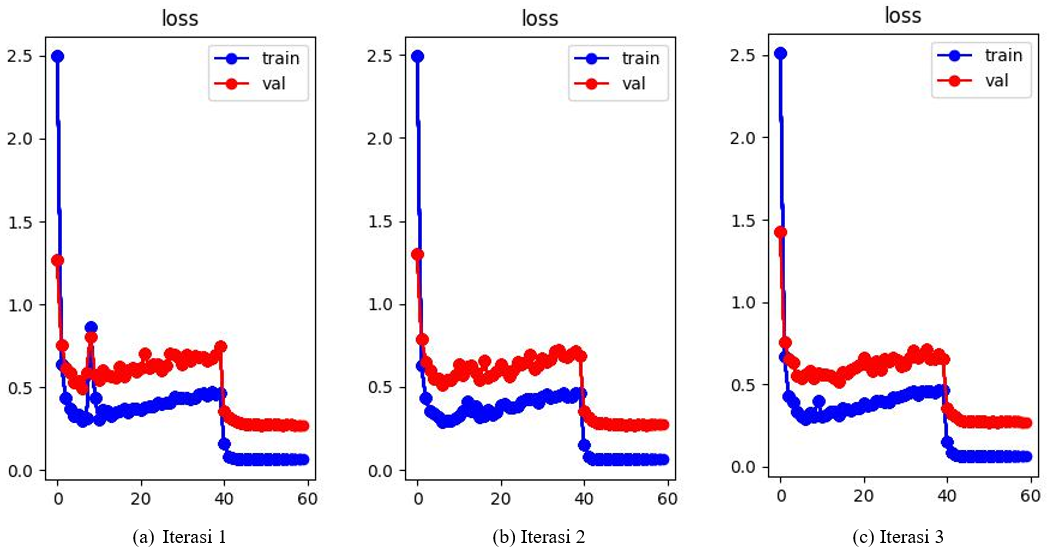
\includegraphics[scale=0.55]{gambar/Train SwinV1 Loss.png}
  % Keterangan gambar yang diinputkan
  \caption{Grafik Loss Setiap Iterasi Swin Transformer V1 Parameter 1}
  % Label referensi dari gambar yang diinputkan
  \label{fig:grafiklossdantop1errdariswinv1parameter1iterasi1}
\end{figure}

\begin{figure}[ht]
  \centering
  % Nama dari file gambar yang diinputkan
  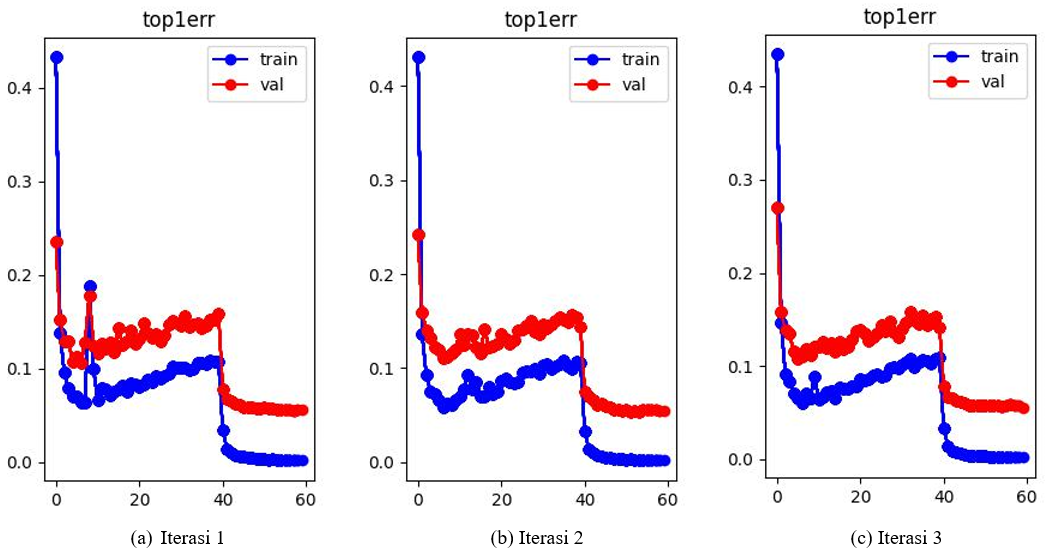
\includegraphics[scale=0.55]{gambar/Train SwinV1 Top1Err.png}
  % Keterangan gambar yang diinputkan
  \caption{Grafik Top 1 Error Setiap Iterasi Swin Transformer V1 Parameter 1}
  % Label referensi dari gambar yang diinputkan
  \label{fig:grafiklossdantop1errdariswinv1parameter1iterasi2}
\end{figure}

% Selain gambar grafik diatas, diperoleh pula nilai mAP, rank@1, rank@5, rank@10 dari proses 
% \emph{Testing} pada masing-masing iterasi. Dari tiga kali iterasi tersebut, maka didapatkan 
% rata-rata dari model Swin Transformer V1 Parameter 1. Seluruh nilai iterasi dan rata-ratanya 
% dapat dilihat pada tabel 4.1.
% Diperoleh pula nilai mAP, rank@1, rank@5, rank@10 dari proses \emph{Testing} pada 
% masing-masing iterasi. Seluruh nilai tersebut dapat dilihat di tabel 4.2.

\begin{table}[h!]
  \begin{center}
  \caption{Nilai mAP, Rank@1, Rank@5, dan Rank@10 Swin Transformer V1 Parameter 1}
  \label{tb:NilaimAP,Rank1,Rank5,danRank10ModelSwinTransformerV1Parameter1}
  \begin{tabular}{|l|l|l|l|l|}
      \hline
      \textit{ } & \begin{tabular}[c]{@{}l@{}}\textbf{mAP}\end{tabular} & \begin{tabular}[c]{@{}l@{}}\textbf{Rank@1}\end{tabular} & \begin{tabular}[c]{@{}l@{}}\textbf{Rank@5}\end{tabular} & \begin{tabular}[c]{@{}l@{}}\textbf{Rank@10}\end{tabular}\\ \hline
      \textit{\textbf{Iterasi 1}} & \begin{tabular}[c]{@{}l@{}}0.667091\end{tabular} & \begin{tabular}[c]{@{}l@{}}0.622199\end{tabular} & \begin{tabular}[c]{@{}l@{}}0.820704\end{tabular} & \begin{tabular}[c]{@{}l@{}}0.870153\end{tabular}\\ \hline
      \textit{\textbf{Iterasi 2}} & \begin{tabular}[c]{@{}l@{}}0.667997\end{tabular} & \begin{tabular}[c]{@{}l@{}}0.621487\end{tabular} & \begin{tabular}[c]{@{}l@{}}0.827819\end{tabular} & \begin{tabular}[c]{@{}l@{}}0.869086\end{tabular}\\ \hline
      \textit{\textbf{Iterasi 3}} & \begin{tabular}[c]{@{}l@{}}\textbf{0.670210}\end{tabular} & \begin{tabular}[c]{@{}l@{}}\textbf{0.623621}\end{tabular} & \begin{tabular}[c]{@{}l@{}}\textbf{0.829598}\end{tabular} & \begin{tabular}[c]{@{}l@{}}\textbf{0.872643}\end{tabular}\\ \hline
      \textit{\textbf{Rata-Rata}} & \begin{tabular}[c]{@{}l@{}}0.668432\end{tabular} & \begin{tabular}[c]{@{}l@{}}0.622435\end{tabular} & \begin{tabular}[c]{@{}l@{}}0.826040\end{tabular} & \begin{tabular}[c]{@{}l@{}}0.870627\end{tabular}\\ \hline
  \end{tabular}
  \end{center}
\end{table}

\subsection{Swin Transformer V2 Parameter 1}

Pada Swin Transformer V2 parameter 1, hyper-parameter yang ditentukan yaitu sebagai berikut:

\begin{itemize}[nolistsep]
  \item Epoch = 60
  \item Batch Size = 32
  \item Random Erasing Probability = 0
  \item Learning Rate = 0.05
  \item Warm Epoch = 0
\end{itemize}

% Dari \emph{training} dan \emph{validation}, didapatkan nilai Akurasi, nilai dan grafik loss, 
% serta grafik Top 1 Error yang dapat dilihat pada tabel 4.3, gambar 4.3, dan gambar 4.4.

Dengan menggunakan hyper-parameter yang ditentukan seperti diatas, dilakukan tiga kali iterasi 
\emph{training} dan \emph{validation} dengan tujuan untuk mendapatkan iterasi dengan nilai mAP \linebreak dan 
rank@1 terbaik untuk model Swin Transformer V2 Parameter 1. Hasil Akurasi, loss, dan Top 1 Error 
pada tahap \emph{training} dan \emph{validation} dapat dilihat pada tabel 4.3, gambar 4.3, dan gambar 4.4.

% Dengan menggunakan hyper-parameter yang ditentukan diatas, didapatkan nilai Akurasi, nilai 
% dan grafik loss, serta grafik Top 1 Error pada tahap \emph{training} dan \emph{validation} 
% yang dapat dilihat pada tabel 4.3, gambar 4.3, dan gambar 4.4.

\begin{table}[h!]
  \begin{center}
  \caption{Nilai Akurasi dan Loss Setiap Iterasi Swin Transformer V2 Parameter 1}
  \label{tb:NilaiakurasidanlossModelSwinTransformerV2Parameter1}
  \begin{tabular}{|l|l|l|l|l|}
      \hline
      \textit{ } & \begin{tabular}[c]{@{}l@{}}\textbf{Train Accuracy}\end{tabular} & \begin{tabular}[c]{@{}l@{}}\textbf{Train Loss}\end{tabular} & \begin{tabular}[c]{@{}l@{}}\textbf{Validation Accuracy}\end{tabular} & \begin{tabular}[c]{@{}l@{}}\textbf{Validation Loss}\end{tabular}\\ \hline
      \textit{\textbf{Iterasi 1}} & \begin{tabular}[c]{@{}l@{}}0.9993\end{tabular} & \begin{tabular}[c]{@{}l@{}}0.0460\end{tabular} & \begin{tabular}[c]{@{}l@{}}0.9530\end{tabular} & \begin{tabular}[c]{@{}l@{}}0.2485\end{tabular}\\ \hline
      \textit{\textbf{Iterasi 2}} & \begin{tabular}[c]{@{}l@{}}0.9993\end{tabular} & \begin{tabular}[c]{@{}l@{}}0.0462\end{tabular} & \begin{tabular}[c]{@{}l@{}}0.9567\end{tabular} & \begin{tabular}[c]{@{}l@{}}0.2361\end{tabular}\\ \hline
      \textit{\textbf{Iterasi 3}} & \begin{tabular}[c]{@{}l@{}}0.9995\end{tabular} & \begin{tabular}[c]{@{}l@{}}0.0458\end{tabular} & \begin{tabular}[c]{@{}l@{}}0.9563\end{tabular} & \begin{tabular}[c]{@{}l@{}}0.2400\end{tabular}\\ \hline
  \end{tabular}
  \end{center}
\end{table}

% Selain nilai akurasi dan loss, diperoleh pula grafik loss, top 1 Error, nilai mAP, rank@1, 
% rank@5, rank@10 dari proses \emph{Testing} dan \emph{validation} pada masing-masing iterasi. 
% Grafik dan nilai tersebut dapat dilihat pada gambar 4.3, gambar 4.4, dan tabel 4.4.

% Dengan melakukan tiga kali iterasi menggunakan hyper-parameter yang disebutkan diatas, maka didapatkan hasil berupa grafik nilai loss dan top 1 error dari proses \emph{training} dan \emph{validation} untuk model Swin Transformer V2 
% parameter 1 yang dapat dilihat pada gambar 4.3, dan gambar 4.4. Tiga kali iterasi dilakukan untuk mendapatkan 
% hasil terbaik dari model Swin Transformer V2 parameter 1.
% \\
% \\

\begin{figure}[h!]
  \centering
  % Nama dari file gambar yang diinputkan
  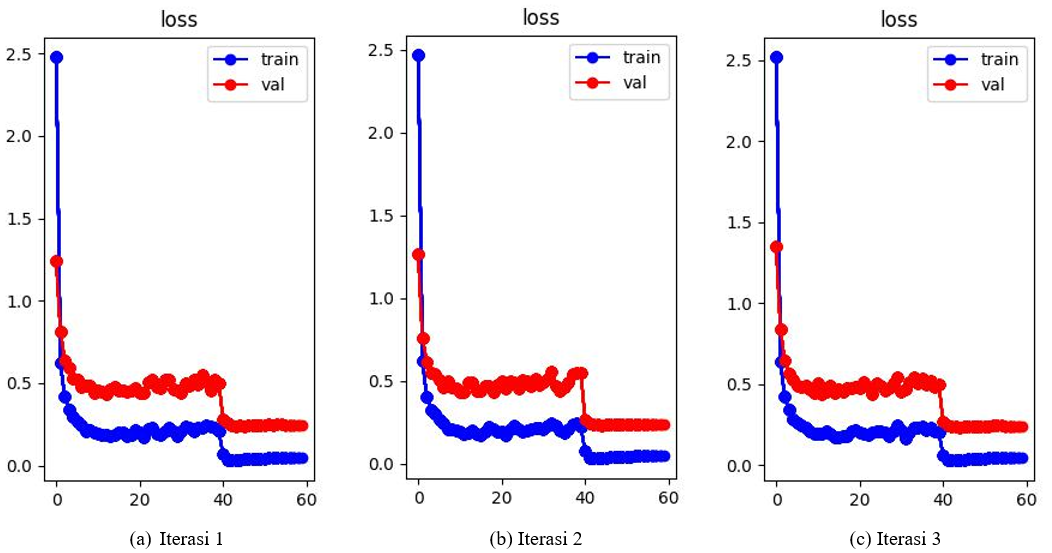
\includegraphics[scale=0.55]{gambar/Train SwinV2 Loss.png}
  % Keterangan gambar yang diinputkan
  \caption{Grafik Loss Setiap Iterasi Swin Transformer V2 Parameter 1}
  % Label referensi dari gambar yang diinputkan
  \label{fig:grafiklossdantop1errdariprosestrainingdanvalidationswinv2iterasi1}
\end{figure}

\begin{figure}[h!]
  \centering
  % Nama dari file gambar yang diinputkan
  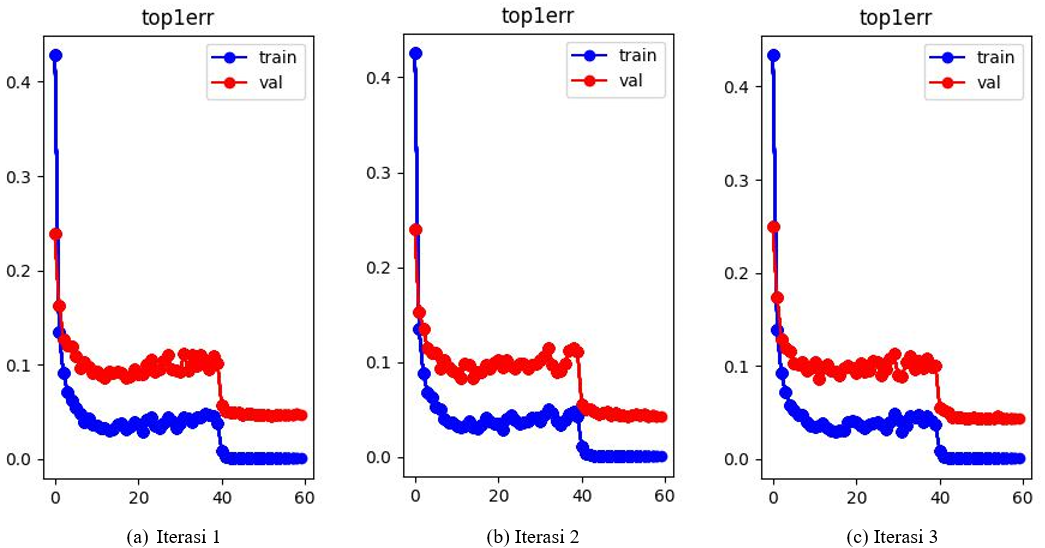
\includegraphics[scale=0.55]{gambar/Train SwinV2 Top1Err.png}
  % Keterangan gambar yang diinputkan
  \caption{Grafik Top 1 Error Setiap Iterasi Swin Transformer V2 Parameter 1}
  % Label referensi dari gambar yang diinputkan
  \label{fig:grafiklossdantop1errdariprosestrainingdanvalidationswinv2iterasi2}
\end{figure}

Selain nilai akurasi, loss, dan Top 1 Error, diperoleh pula nilai mAP, rank@1, 
rank@5, rank@10 dari proses \emph{Testing} dan \emph{validation} pada 
masing-masing iterasi. Grafik dan nilai tersebut dapat dilihat pada tabel 4.4.

% Diperoleh pula nilai mAP, rank@1, rank@5, rank@10 dari proses \emph{Testing} pada 
% masing-masing iterasi. Seluruh nilai tersebut dapat dilihat di tabel 4.5.

\begin{table}[h!]
  \begin{center}
  \caption{Nilai mAP, Rank@1, Rank@5, dan Rank@10 Swin Transformer V2 Parameter 1}
  \label{tb:NilaimAP,Rank1,Rank5,danRank10ModelSwinTransformerV2Parameter1}
  \begin{tabular}{|l|l|l|l|l|}
      \hline
      \textit{ } & \begin{tabular}[c]{@{}l@{}}\textbf{mAP}\end{tabular} & \begin{tabular}[c]{@{}l@{}}\textbf{Rank@1}\end{tabular} & \begin{tabular}[c]{@{}l@{}}\textbf{Rank@5}\end{tabular} & \begin{tabular}[c]{@{}l@{}}\textbf{Rank@10}\end{tabular}\\ \hline
      \textit{\textbf{Iterasi 1}} & \begin{tabular}[c]{@{}l@{}}\textbf{0.725377}\end{tabular} & \begin{tabular}[c]{@{}l@{}}\textbf{0.686233}\end{tabular} & \begin{tabular}[c]{@{}l@{}}0.857346\end{tabular} & \begin{tabular}[c]{@{}l@{}}0.895411\end{tabular}\\ \hline
      \textit{\textbf{Iterasi 2}} & \begin{tabular}[c]{@{}l@{}}0.719978\end{tabular} & \begin{tabular}[c]{@{}l@{}}0.678762\end{tabular} & \begin{tabular}[c]{@{}l@{}}\textbf{0.863750}\end{tabular} & \begin{tabular}[c]{@{}l@{}}\textbf{0.903949}\end{tabular}\\ \hline
      \textit{\textbf{Iterasi 3}} & \begin{tabular}[c]{@{}l@{}}0.715753\end{tabular} & \begin{tabular}[c]{@{}l@{}}0.674493\end{tabular} & \begin{tabular}[c]{@{}l@{}}0.854856\end{tabular} & \begin{tabular}[c]{@{}l@{}}0.897901\end{tabular}\\ \hline
      \textit{\textbf{Rata-Rata}} & \begin{tabular}[c]{@{}l@{}}0.720369\end{tabular} & \begin{tabular}[c]{@{}l@{}}0.679829\end{tabular} & \begin{tabular}[c]{@{}l@{}}0.858651\end{tabular} & \begin{tabular}[c]{@{}l@{}}0.899087\end{tabular}\\ \hline
  \end{tabular}
  \end{center}
\end{table}

\subsection{Swin Transformer V1 Parameter 2}

Pada Swin Transformer V1 parameter 2, hyper-parameter yang ditentukan yaitu sebagai berikut:

\begin{itemize}[nolistsep]
  \item Epoch = 60
  \item Batch Size = 16
  \item Random Erasing Probability = 0.5
  \item Learning Rate = 0.01
  \item Warm Epoch = 5
\end{itemize}

Dengan menggunakan hyper-parameter yang ditentukan seperti diatas, dilakukan tiga kali iterasi 
\emph{training} dan \emph{validation} dengan tujuan untuk mendapatkan iterasi dengan nilai mAP dan 
rank@1 terbaik untuk model Swin Transformer V1 Parameter 2. Hasil Akurasi dan loss pada tahap 
\emph{training} dan \emph{validation} dapat dilihat pada tabel 4.5.

\begin{table}[h!]
  \begin{center}
  \caption{Nilai Akurasi dan Loss Setiap Iterasi Swin Transformer V1 Parameter 2}
  \label{tb:NilaiakurasidanlossModelSwinTransformerV1Parameter2}
  \begin{tabular}{|l|l|l|l|l|}
      \hline
      \textit{ } & \begin{tabular}[c]{@{}l@{}}\textbf{Train Accuracy}\end{tabular} & \begin{tabular}[c]{@{}l@{}}\textbf{Train Loss}\end{tabular} & \begin{tabular}[c]{@{}l@{}}\textbf{Validation Accuracy}\end{tabular} & \begin{tabular}[c]{@{}l@{}}\textbf{Validation Loss}\end{tabular}\\ \hline
      \textit{\textbf{Iterasi 1}} & \begin{tabular}[c]{@{}l@{}}0.9979\end{tabular} & \begin{tabular}[c]{@{}l@{}}0.1139\end{tabular} & \begin{tabular}[c]{@{}l@{}}0.9571\end{tabular} & \begin{tabular}[c]{@{}l@{}}0.1969\end{tabular}\\ \hline
      \textit{\textbf{Iterasi 2}} & \begin{tabular}[c]{@{}l@{}}0.9980\end{tabular} & \begin{tabular}[c]{@{}l@{}}0.1196\end{tabular} & \begin{tabular}[c]{@{}l@{}}0.9578\end{tabular} & \begin{tabular}[c]{@{}l@{}}0.1897\end{tabular}\\ \hline
      \textit{\textbf{Iterasi 3}} & \begin{tabular}[c]{@{}l@{}}0.9985\end{tabular} & \begin{tabular}[c]{@{}l@{}}0.1180\end{tabular} & \begin{tabular}[c]{@{}l@{}}0.9563\end{tabular} & \begin{tabular}[c]{@{}l@{}}0.1847\end{tabular}\\ \hline
  \end{tabular}
  \end{center}
\end{table}

\begin{figure}[h!]
  \centering
  % Nama dari file gambar yang diinputkan
  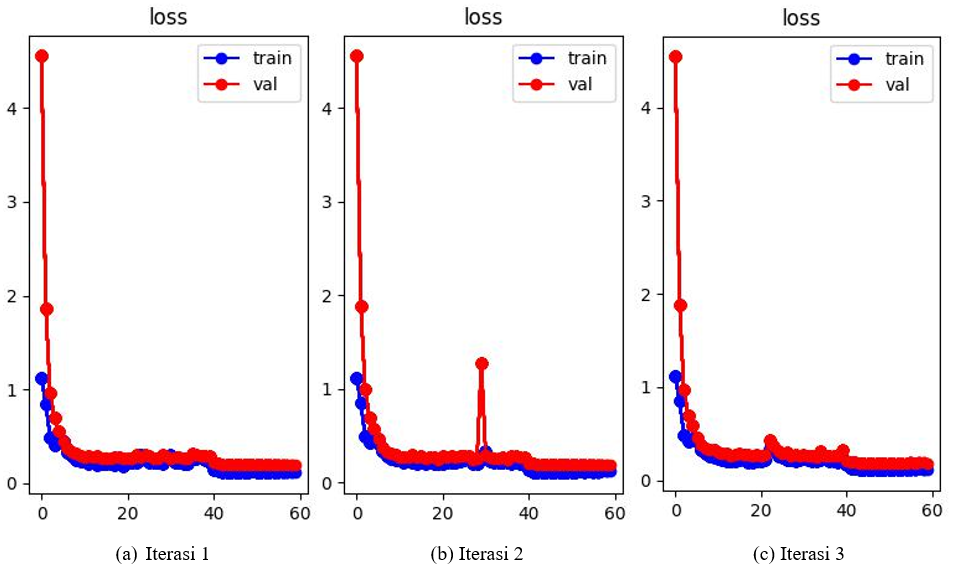
\includegraphics[scale=0.55]{gambar/Train SwinV1CP1 Loss.png}
  % Keterangan gambar yang diinputkan
  \caption{Grafik Loss Setiap Iterasi Swin Transformer V1 Parameter 2}
  % Label referensi dari gambar yang diinputkan
  \label{fig:grafiklossdariswinv1parameter2}
\end{figure}

\begin{figure}[ht]
  \centering
  % Nama dari file gambar yang diinputkan
  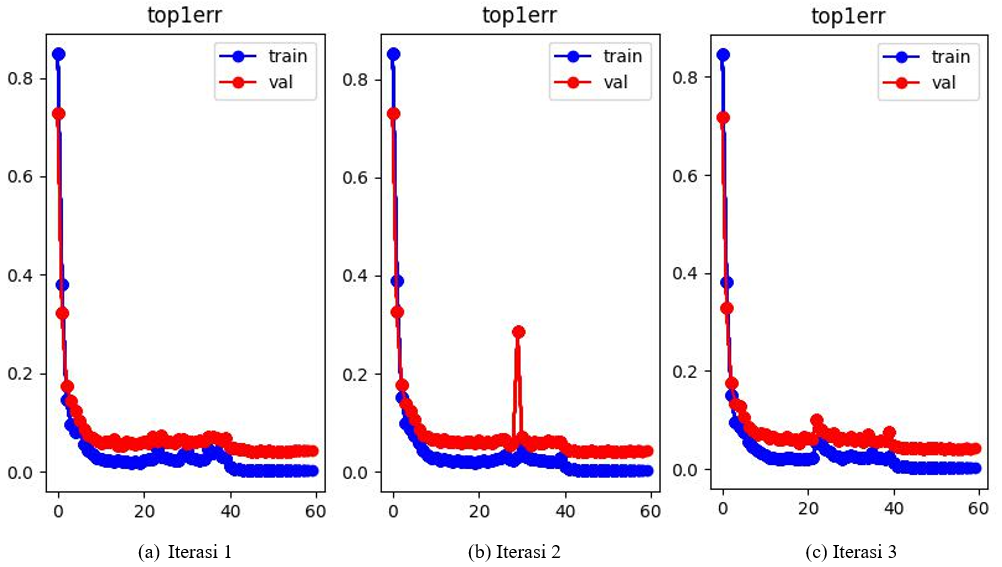
\includegraphics[scale=0.55]{gambar/Train SwinV1CP1 Top1Err.png}
  % Keterangan gambar yang diinputkan
  \caption{Grafik Top 1 Error Setiap Iterasi Swin Transformer V1 Parameter 2}
  % Label referensi dari gambar yang diinputkan
  \label{fig:grafiktop1errdariswinv1parameter1}
\end{figure}

% Selain gambar grafik diatas, diperoleh pula nilai mAP, rank@1, rank@5, rank@10 dari proses 
% \emph{Testing} pada masing-masing iterasi. Dari tiga kali iterasi tersebut, maka didapatkan 
% rata-rata dari model Swin Transformer V1 Parameter 1. Seluruh nilai iterasi dan rata-ratanya 
% dapat dilihat pada tabel 4.1.
% Diperoleh pula nilai mAP, rank@1, rank@5, rank@10 dari proses \emph{Testing} pada 
% masing-masing iterasi. Seluruh nilai tersebut dapat dilihat di tabel 4.2.

\begin{table}[h!]
  \begin{center}
  \caption{Nilai mAP, Rank@1, Rank@5, dan Rank@10 Swin Transformer V1 Parameter 2}
  \label{tb:NilaimAP,Rank1,Rank5,danRank10ModelSwinTransformerV1Parameter2}
  \begin{tabular}{|l|l|l|l|l|}
      \hline
      \textit{ } & \begin{tabular}[c]{@{}l@{}}\textbf{mAP}\end{tabular} & \begin{tabular}[c]{@{}l@{}}\textbf{Rank@1}\end{tabular} & \begin{tabular}[c]{@{}l@{}}\textbf{Rank@5}\end{tabular} & \begin{tabular}[c]{@{}l@{}}\textbf{Rank@10}\end{tabular}\\ \hline
      \textit{\textbf{Iterasi 1}} & \begin{tabular}[c]{@{}l@{}}0.745984\end{tabular} & \begin{tabular}[c]{@{}l@{}}0.704731\end{tabular} & \begin{tabular}[c]{@{}l@{}}0.887229\end{tabular} & \begin{tabular}[c]{@{}l@{}}0.926361\end{tabular}\\ \hline
      \textit{\textbf{Iterasi 2}} & \begin{tabular}[c]{@{}l@{}}\textbf{0.751921}\end{tabular} & \begin{tabular}[c]{@{}l@{}}\textbf{0.711135}\end{tabular} & \begin{tabular}[c]{@{}l@{}}\textbf{0.892209}\end{tabular} & \begin{tabular}[c]{@{}l@{}}0.933120\end{tabular}\\ \hline
      \textit{\textbf{Iterasi 3}} & \begin{tabular}[c]{@{}l@{}}0.750978\end{tabular} & \begin{tabular}[c]{@{}l@{}}0.709712\end{tabular} & \begin{tabular}[c]{@{}l@{}}0.891498\end{tabular} & \begin{tabular}[c]{@{}l@{}}\textbf{0.934899}\end{tabular}\\ \hline
      \textit{\textbf{Rata-Rata}} & \begin{tabular}[c]{@{}l@{}}0.749627\end{tabular} & \begin{tabular}[c]{@{}l@{}}0.708526\end{tabular} & \begin{tabular}[c]{@{}l@{}}0.890312\end{tabular} & \begin{tabular}[c]{@{}l@{}}0.93146\end{tabular}\\ \hline
  \end{tabular}
  \end{center}
\end{table}

\subsection{Swin Transformer V2 Parameter 2}

Pada Swin Transformer V2 parameter 2, hyper-parameter yang ditentukan yaitu sebagai berikut:

\begin{itemize}[nolistsep]
  \item Epoch = 60
  \item Batch Size = 16
  \item Random Erasing Probability = 0.5
  \item Learning Rate = 0.01
  \item Warm Epoch = 5
\end{itemize}

\begin{figure}[ht]
  \centering
  % Nama dari file gambar yang diinputkan
  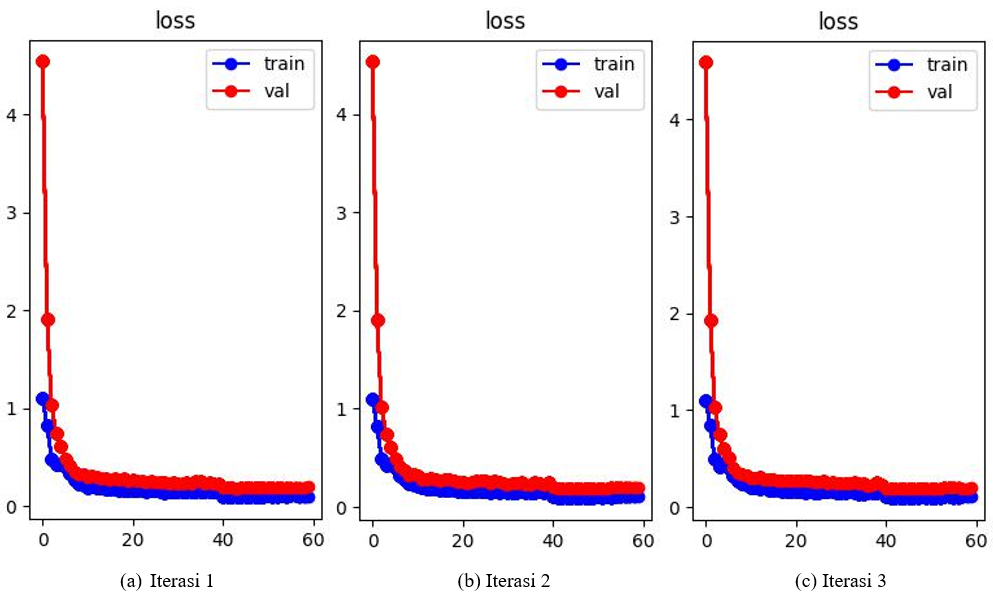
\includegraphics[scale=0.55]{gambar/Train SwinV2CP1 Loss.png}
  % Keterangan gambar yang diinputkan
  \caption{Grafik Loss Setiap Iterasi Swin Transformer V2 Parameter 2}
  % Label referensi dari gambar yang diinputkan
  \label{fig:grafiklossdariswinv2parameter2}
\end{figure}

\begin{figure}[ht]
  \centering
  % Nama dari file gambar yang diinputkan
  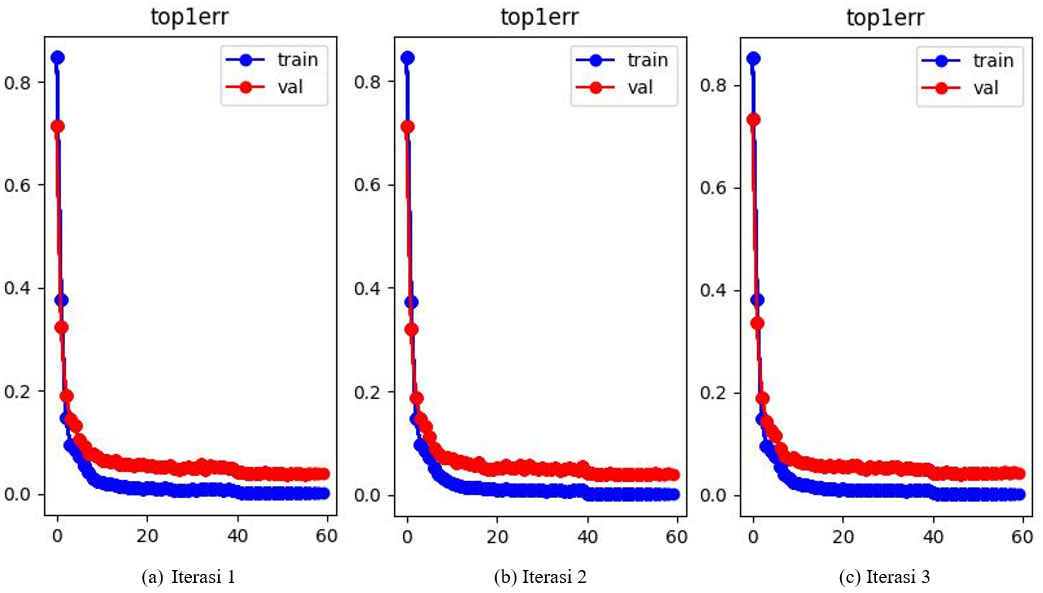
\includegraphics[scale=0.55]{gambar/Train SwinV2CP1 Top1Err.png}
  % Keterangan gambar yang diinputkan
  \caption{Grafik Top 1 Error Setiap Iterasi Swin Transformer V2 Parameter 2}
  % Label referensi dari gambar yang diinputkan
  \label{fig:grafiktop1errdariswinv2parameter2}
\end{figure}

Selain gambar grafik diatas, diperoleh pula nilai mAP, rank@1, rank@5, rank@10 dari proses 
\emph{Testing} pada masing-masing iterasi. Dari tiga kali iterasi tersebut, maka didapatkan 
rata-rata dari model Swin Transformer V2 Parameter 2. Seluruh nilai iterasi dan rata-ratanya 
dapat dilihat pada tabel 4.4.
% Diperoleh pula nilai mAP, rank@1, rank@5, rank@10 dari proses \emph{Testing} pada 
% masing-masing iterasi. Seluruh nilai tersebut dapat dilihat di tabel 4.2.

\begin{table}[h!]
  \begin{center}
  \caption{Nilai mAP, Rank@1, Rank@5, dan Rank@10 Swin Transformer V2 Parameter 2}
  \label{tb:NilaimAP,Rank1,Rank5,danRank10ModelSwinTransformerV2Parameter2}
  \begin{tabular}{|l|l|l|l|l|}
      \hline
      \textit{ } & \begin{tabular}[c]{@{}l@{}}\textbf{mAP}\end{tabular} & \begin{tabular}[c]{@{}l@{}}\textbf{Rank@1}\end{tabular} & \begin{tabular}[c]{@{}l@{}}\textbf{Rank@5}\end{tabular} & \begin{tabular}[c]{@{}l@{}}\textbf{Rank@10}\end{tabular}\\ \hline
      \textit{\textbf{Iterasi 1}} & \begin{tabular}[c]{@{}l@{}}0.750173\end{tabular} & \begin{tabular}[c]{@{}l@{}}0.710423\end{tabular} & \begin{tabular}[c]{@{}l@{}}\textbf{0.890786}\end{tabular} & \begin{tabular}[c]{@{}l@{}}0.929918\end{tabular}\\ \hline
      \textit{\textbf{Iterasi 2}} & \begin{tabular}[c]{@{}l@{}}0.750367\end{tabular} & \begin{tabular}[c]{@{}l@{}}0.710068\end{tabular} & \begin{tabular}[c]{@{}l@{}}0.889363\end{tabular} & \begin{tabular}[c]{@{}l@{}}0.925294\end{tabular}\\ \hline
      \textit{\textbf{Iterasi 3}} & \begin{tabular}[c]{@{}l@{}}\textbf{0.751293}\end{tabular} & \begin{tabular}[c]{@{}l@{}}\textbf{0.711135}\end{tabular} & \begin{tabular}[c]{@{}l@{}}0.889719\end{tabular} & \begin{tabular}[c]{@{}l@{}}\textbf{0.930985}\end{tabular}\\ \hline
      \textit{\textbf{Rata-Rata}} & \begin{tabular}[c]{@{}l@{}}0.750611\end{tabular} & \begin{tabular}[c]{@{}l@{}}0.710542\end{tabular} & \begin{tabular}[c]{@{}l@{}}0.889956\end{tabular} & \begin{tabular}[c]{@{}l@{}}0.928732\end{tabular}\\ \hline
  \end{tabular}
  \end{center}
\end{table}

\section{Analisa Hasil}
\label{sec:analisahasil}

% Dari tabel 4.1, tabel 4.2, serta grafik loss dan top 1 error yang ditampilkan pada bagian 4.1.1 dan 4.1.2, dapat diteliti 
% hasil model terbaik dari proses \emph{training} dan \emph{validation}. Iterasi dari masing-masing jenis model akan 
% mengambil hasil epoch terbaik dari proses \emph{training} dan \emph{validation}, sehingga hasil yang digunakan belum 
% tentu merupakan epoch terakhir dari proses \emph{training} dan \emph{validation}. Penjelasan terkait hasil dari setiap 
% jenis model yaitu sebagai berikut.

Dari tabel 4.1, tabel 4.2, serta grafik loss dan top 1 error yang ditampilkan pada bagian 4.1.1 dan 4.1.2, dapat diteliti 
hasil model terbaik dari proses \emph{training} dan \emph{validation}. Setiap jenis model re-identifikasi mobil akan 
mengambil hasil iterasi terbaik dari proses \emph{training} dan \emph{validation}, sehingga hasil yang digunakan pada 
pengujian belum tentu merupakan iterasi terakhir dari proses \emph{training} dan \emph{validation}. Penjelasan terkait 
hasil dari setiap jenis model yaitu sebagai berikut.

\subsection{Swin Transformer V1 Parameter 1}

Pada model Swin Transformer V1 parameter 1, model yang digunakan yaitu Swin-B (\emph{Base}), yang merupakan bentuk 
dasar dari arsitektur Swin Transformer. Dari tiga kali iterasi yang dilakukan, didapatkan data bahwa rata-rata nilai 
mAP (\emph{Mean Average Precision}) untuk model Swin Transformer V1 parameter 1 sebesar 0,668 atau 66,8\%. Dan untuk 
rank@1, rank@5, dan rank@10 berturut-turut sebesar 62,2\%, 82,6\%, dan 87,1\%. 

Berdasarkan Tabel 4.1, iterasi ketiga menjadi iterasi dengan hasil terbaik untuk model Swin Transformer V1 parameter 1. 
Hal ini didasarkan pada nilai mAP yang didapat yaitu sebesar 0.67 atau 67\%. Nilai tersebut 0,2\% lebih besar dari 
mAP rata-rata. Selain itu rank@1 yang didapat sebesar 62,4\% atau 0,2\% lebih besar dari rank@1 rata-rata. Rank@5 sebesar 
82,9\% atau 0,4\% lebih besar dari rank@5 rata-rata. Dan rank@10 sebesar 87,3\% atau 0,2\% lebih besar dari rank@10 
rata-rata.

\subsection{Swin Transformer V2 Parameter 1}

Pada model Swin Transformer V2 parameter 1, model yang digunakan yaitu Swin-B (\emph{Base}), yang merupakan bentuk 
dasar dari arsitektur Swin Transformer V2. Dari tiga kali iterasi yang dilakukan, didapatkan data bahwa rata-rata nilai 
mAP (\emph{Mean Average Precision}) untuk model Swin Transformer V2 parameter 1 sebesar 0,72 atau 72\%. Dan untuk 
rank@1, rank@5, dan rank@10 berturut-turut sebesar 67,9\%, 85,8\%, dan 89,9\%. 

Berdasarkan Tabel 4.2, iterasi pertama menjadi iterasi dengan hasil terbaik untuk model Swin Transformer V2 parameter 1. 
Hal ini didasarkan pada nilai mAP yang didapat yaitu sebesar 0.725 atau 72,5\%. Nilai tersebut 0,5\% lebih besar dari 
mAP rata-rata. Selain itu rank@1 yang didapat sebesar 68,6\% atau 0,7\% lebih besar dari rank@1 rata-rata. Namun 
Rank@5 memiliki nilai sebesar 85,7\% atau 0,1\% lebih kecil dari rank@5 rata-rata. Dan rank@10 sebesar 89,5\% atau 0,4\% 
lebih kecil dari rank@10 rata-rata.

\section{Skenario Pengujian}
\label{sec:skenariopengujian}

Pengujian dilakukan pada setiap model re-identifikasi mobil dengan iterasi terbaik pada masing-masing modelnya. Setiap 
model memiliki iterasi terbaiknya masing-masing yang telah dijelaskan pada bagian 4.2.1 dan 4.2.2. Dari hasil \emph{training} 
dan \emph{validation}, maka model dapat dilakukan \emph{testing} menggunakan data \emph{test} yang telah tersedia dari 
dataset VRIC.

Pengujian dilakukan dengan cara memasukkan sebuah gambar kueri ke dalam model re-identifikasi mobil. Model yang sudah memiliki 
galeri berisi kumpulan gambar mobil kemudian akan mencari gambar dengan objek (mobil) yang memiliki kemiripan dengan gambar 
kueri di galeri. Beberapa gambar yang memiliki kemiripan tertinggi dengan kueri kemudian akan dibuat list tingkat kemiripan 
gambar galeri berdasarkan gambar kueri. Dikarenakan jumlah gambar kueri yang mencapai ribuan, maka hanya akan dicantumkan 
beberapa sampel dari pengujian yang dilakukan. Berikut merupakan hasil pengujian model re-identifikasi mobil.

\subsection{Pengujian Pertama}

Model Swin Transformer V1 parameter 1 menggunakan iterasi ketiga sebagai model pengujian re-identifikasi mobil. Pengujian pertama
re-identifikasi mobil dari Swin Transformer V1 parameter 1 dapat dilihat pada gambar 4.5.

\begin{figure}[ht]
  \centering
  % Nama dari file gambar yang diinputkan
  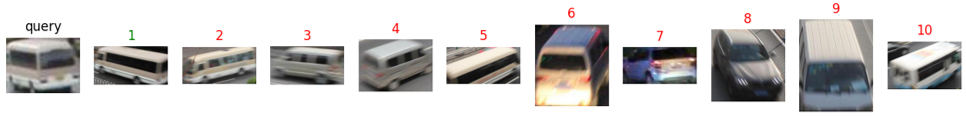
\includegraphics[scale=0.6]{gambar/Que8V1P1IT3.png}
  % Keterangan gambar yang diinputkan
  \caption{Hasil Pengujian Pertama pada Model Swin Transformer V1 Parameter 1}
  % Label referensi dari gambar yang diinputkan
  \label{fig:hasilpengujianpertamapadamodelswintransformerv1param1}
\end{figure}

Model Swin Transformer V2 parameter 1 menggunakan iterasi pertama sebagai model pengujian re-identifikasi mobil. Pengujian pertama
re-identifikasi mobil dari Swin Transformer V2 parameter 1 dapat dilihat pada gambar 4.6.

\begin{figure}[ht]
  \centering
  % Nama dari file gambar yang diinputkan
  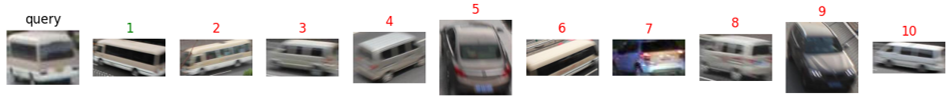
\includegraphics[scale=0.6]{gambar/Que8V2P1IT1.png}
  % Keterangan gambar yang diinputkan
  \caption{Hasil Pengujian Pertama pada Model Swin Transformer V2 Parameter 1}
  % Label referensi dari gambar yang diinputkan
  \label{fig:hasilpengujianpertamapadamodelswintransformerv2param1}
\end{figure}

\subsection{Pengujian Kedua}

Pengujian kedua re-identifikasi mobil dari Swin Transformer V1 parameter 1 dapat dilihat pada gambar 4.7.

\begin{figure}[ht]
  \centering
  % Nama dari file gambar yang diinputkan
  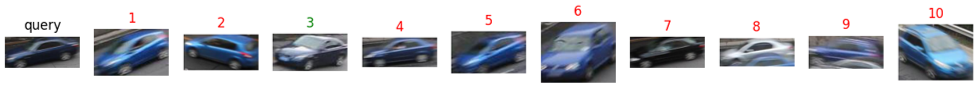
\includegraphics[scale=0.6]{gambar/qUE57v1P1IT3.png}
  % Keterangan gambar yang diinputkan
  \caption{Hasil Pengujian Kedua pada Model Swin Transformer V1 Parameter 1}
  % Label referensi dari gambar yang diinputkan
  \label{fig:hasilpengujiankeduapadamodelswintransformerv1param1}
\end{figure}

Pengujian kedua re-identifikasi mobil dari Swin Transformer V2 parameter 1 dapat dilihat pada gambar 4.8.

\begin{figure}[h!]
  \centering
  % Nama dari file gambar yang diinputkan
  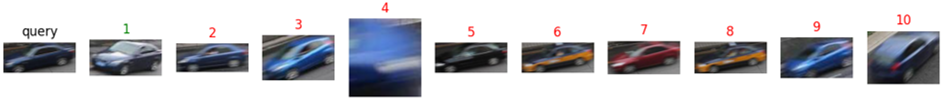
\includegraphics[scale=0.6]{gambar/Que57V2P1IT1.png}
  % Keterangan gambar yang diinputkan
  \caption{Hasil Pengujian Kedua pada Model Swin Transformer V2 Parameter 1}
  % Label referensi dari gambar yang diinputkan
  \label{fig:hasilpengujiankeduapadamodelswintransformerv2param1}
\end{figure}

\subsection{Pengujian Ketiga}

Pengujian ketiga re-identifikasi mobil dari Swin Transformer V1 parameter 1 dapat dilihat pada gambar 4.9. \\
\\
\\

\begin{figure}[ht]
  \centering
  % Nama dari file gambar yang diinputkan
  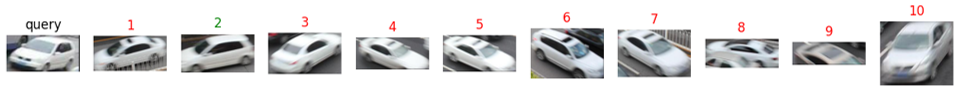
\includegraphics[scale=0.6]{gambar/Que61V1P1IT3.png}
  % Keterangan gambar yang diinputkan
  \caption{Hasil Pengujian Ketiga pada Model Swin Transformer V1 Parameter 1}
  % Label referensi dari gambar yang diinputkan
  \label{fig:hasilpengujianketigapadamodelswintransformerv1param1}
\end{figure}

Pengujian ketiga re-identifikasi mobil dari Swin Transformer V2 parameter 1 dapat dilihat pada gambar 4.10.

\begin{figure}[ht]
  \centering
  % Nama dari file gambar yang diinputkan
  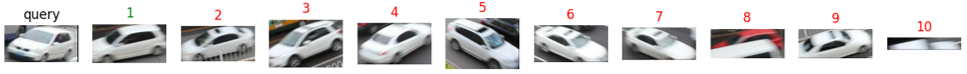
\includegraphics[scale=0.6]{gambar/Que61V2P1IT1.png}
  % Keterangan gambar yang diinputkan
  \caption{Hasil Pengujian Ketiga pada Model Swin Transformer V2 Parameter 1}
  % Label referensi dari gambar yang diinputkan
  \label{fig:hasilpengujianketigapadamodelswintransformerv2param1}
\end{figure}

\section{Analisa Pengujian}
\label{sec:analisapengujian}

Pengujian dilakukan dengan membandingkan ketepatan re-identifikasi mobil dari masing-masing model menggunakan 
data \emph{test} dari dataset VRIC. Berdasarkan gambar-gambar pada bagian 4.3. dapat terlihat ketepatan 
re-identifikasi dari setiap modelnya ketika diberikan gambar kueri yang sama. 

Pada pengujian pertama dapat terlihat bahwa model Swin Transformer V1 parameter 1 (pada gambar 4.5) 
dan model Swin Transformer V2 parameter 1 (pada gambar 4.6) dengan tepat dapat melakukan re-identifikasi 
ulang sebuah bis.

Pada pengujian kedua, ketika diberikan sebuah gambar kueri mobil berwarna biru tua, model Swin Transformer V1 
parameter 1 (pada gambar 4.7) kurang tepat dalam melakukan re-identifikasi mobil, dimana gambar yang sesuai 
dengan gambar kueri berada pada rank 3. Sementara model Swin Transformer V2 parameter 1 (pada gambar 4.8) dapat 
mengindentifikasi gambar kueri dengan tepat dan gambar dari galeri yang sesuai berada pada rank 1.

Pada pengujian ketiga, ketika diberikan sebuah gambar kueri mobil berwarna putih, model Swin Transformer V1 
parameter 1 (pada gambar 4.8) juga kurang tepat dalam melakukan re-identifikasi mobil, dimana gambar yang sesuai 
dengan gambar kueri berada pada rank 2. Sementara model Swin Transformer V2 parameter 1 (pada gambar 4.9) dengan 
tepat mengindentifikasi gambar kueri dan menaruhnya pada rank 1.

Perbandingan nilai mAP, rank@1, rank@5, dan rank@10 dari setiap model Swin Transformer dapat dilihat pada tabel 
4.3.

\begin{table}[h!]
  \begin{center}
  \caption{Nilai mAP, Rank@1, Rank@5, dan Rank@10 Setiap Model Swin Transformer}
  \label{tb:NilaimAP,Rank1,Rank5,danRank10SetiapModelSwinTransformer}
  \begin{tabular}{|l|l|l|l|l|}
      \hline
      \textit{ } & \begin{tabular}[c]{@{}l@{}}\textbf{mAP}\end{tabular} & \begin{tabular}[c]{@{}l@{}}\textbf{Rank@1}\end{tabular} & \begin{tabular}[c]{@{}l@{}}\textbf{Rank@5}\end{tabular} & \begin{tabular}[c]{@{}l@{}}\textbf{Rank@10}\end{tabular}\\ \hline
      \textit{\textbf{Swin Transformer V1 Parameter 1}} & \begin{tabular}[c]{@{}l@{}}0.670210\end{tabular} & \begin{tabular}[c]{@{}l@{}}0.623621\end{tabular} & \begin{tabular}[c]{@{}l@{}}0.829598\end{tabular} & \begin{tabular}[c]{@{}l@{}}0.872643\end{tabular}\\ \hline
      \textit{\textbf{Swin Transformer V2 Parameter 1}} & \begin{tabular}[c]{@{}l@{}}0.725377\end{tabular} & \begin{tabular}[c]{@{}l@{}}0.686233\end{tabular} & \begin{tabular}[c]{@{}l@{}}0.857346\end{tabular} & \begin{tabular}[c]{@{}l@{}}0.895411\end{tabular}\\ \hline
      \textit{\textbf{Swin Transformer V1 Parameter 2}} & \begin{tabular}[c]{@{}l@{}} \end{tabular} & \begin{tabular}[c]{@{}l@{}} \end{tabular} & \begin{tabular}[c]{@{}l@{}} \end{tabular} & \begin{tabular}[c]{@{}l@{}} \end{tabular}\\ \hline
      \textit{\textbf{Swin Transformer V2 Parameter 2}} & \begin{tabular}[c]{@{}l@{}} \end{tabular} & \begin{tabular}[c]{@{}l@{}} \end{tabular} & \begin{tabular}[c]{@{}l@{}} \end{tabular} & \begin{tabular}[c]{@{}l@{}} \end{tabular}\\ \hline
  \end{tabular}
  \end{center}
\end{table}

Berdasarkan tabel 4.3 dan pengujian-pengujian yang dilakukan sampai saat ini, dapat terlihat bahwa model Swin 
Transformer V1 parameter 1 dapat mengidentifikasi ulang mobil dengan ketepatan satu banding tiga. Sementara 
model Swin Transformer V2 parameter 1 dapat mengindentifikasi ulang mobil dengan ketepatan tiga banding tiga. 
Hal ini menunjukan model Swin Transformer V2 parameter 1 menjadi model re-identifikasi mobil yang memiliki 
hasil terbaik sejauh pengerjaan penelitian ini. 

% Dari pengujian yang \lipsum[1]

% % Contoh pembuatan tabel
% \begin{longtable}{|c|c|c|}
%   \caption{Hasil Pengukuran Energi dan Kecepatan}
%   \label{tb:EnergiKecepatan}                                   \\
%   \hline
%   \rowcolor[HTML]{C0C0C0}
%   \textbf{Energi} & \textbf{Jarak Tempuh} & \textbf{Kecepatan} \\
%   \hline
%   10 J            & 1000 M                & 200 M/s            \\
%   20 J            & 2000 M                & 400 M/s            \\
%   30 J            & 4000 M                & 800 M/s            \\
%   40 J            & 8000 M                & 1600 M/s           \\
%   \hline
% \end{longtable}

% \lipsum[2-4]

\cleardoublepage

% Bab 5 penutup
\chapter{PENUTUP}
\label{chap:penutup}

% Ubah bagian-bagian berikut dengan isi dari penutup

\section{Kesimpulan}
\label{sec:kesimpulan}

Berdasarkan hasil pengujian yang telah dijelaskan pada Bab 4, dapat 
ditarik beberapa kesimpulan sebagai berikut:

\begin{enumerate}[nolistsep]

  \item Pembuatan Model Re-Identifikasi dengan metode Swin Transformer untuk 
  mengidentifikasi ulang mobil berhasil dibuat dengan nilai mAP tertinggi yang didapat 
  di penelitian ini sebesar 75.26\% dan rank@1 tertinggi sebesar 71.22\%.

  \item Dari keseluruhan model yang telah dibuat pada penelitian ini, 
  model terbaik yang dapat digunakan untuk model re-identifikasi mobil adalah 
  Swin Transformer V2 dengan pengaturan parameter 2. Hal ini dibuktikan dengan nilai 
  mAP rata-rata yang didapat sebesar 75.16\% dan rank@1 rata-rata sebesar 71.2\%

  \item Arsitektur Swin Transformer cocok digunakan untuk menyelesaikan permasalahan 
  re-identifikasi kendaraan karena dapat mengidentifikasi citra dengan resolusi yang cukup 
  kecil, sehingga melakukan re-identifikasi dengan sebuah citra dengan objek yang 
  tidak terlalu jelas dapat dilakukan.

  \item Model re-identifikasi mobil yang dibuat di penelitian ini masih belum mengungguli 
  model re-identifikasi dari penelitian terdahulu yang menggunakan VRIC sebagai dataset 
  dan CNN sebagai arsitektur.

\end{enumerate}

\section{Saran}
\label{chap:saran}

Untuk pengembangan lebih lanjut pada penelitian berikutnya atau yang akan datang, \linebreak
penulis memiliki beberapa saran antara lain:

\begin{enumerate}[nolistsep]

  \item Menggunakan Dataset citra yang berasal dari daerah lokal atau berasal dari Indonesia.

  \item Perlunya pembenahan dan pengaturan pada hyper-parameter agar model dapat melakukan 
  re-identifikasi dengan lebih baik.

  \item Mencoba menggunakan varian model lain dari Swin Transformer di penelitian kedepannya.

\end{enumerate}

\cleardoublepage

\chapter*{DAFTAR PUSTAKA}
\addcontentsline{toc}{chapter}{DAFTAR PUSTAKA}
\renewcommand\refname{}
\vspace{2ex}
\renewcommand{\bibname}{}
\begingroup
\def\chapter*#1{}
\printbibliography
\endgroup
\cleardoublepage

% Biografi penulis
\begin{center}
  \Large
  \textbf{BIOGRAFI PENULIS}
\end{center}

\addcontentsline{toc}{chapter}{BIOGRAFI PENULIS}

\vspace{2ex}

\begin{wrapfigure}{L}{0.3\textwidth}
  \centering
  \vspace{-3ex}
  % Ubah file gambar berikut dengan file foto dari mahasiswa
  
\includegraphics[width=0.3\textwidth]{gambar/elon.jpg}
  \vspace{-4ex}
\end{wrapfigure}

% Ubah kalimat berikut dengan biografi dari mahasiswa
\name{}, lahir pada tanggal 14 Mei 2001 di Kota Semarang, Jawa Tengah. Merupakan anak kedua dari 
dua bersaudara. Setelah lulus dari SMAN 1 Semarang, penulis melanjutkan pendidikan ke jenjang 
Perguruan Tinggi di program Strata 1 (S1) Departemen Teknik Komputer, Fakultas Teknologi Elektro 
dan Informatika Cerdas (FTEIC), Institut Teknologi Sepuluh Nopember (ITS) Surabaya. Selama berkuliah, 
penulis mengikuti berbagai kegiatan akademis seperti menjadi asisten laboratorium B401, asisten 
praktikum Rangkaian Digital 2022, menjadi peserta Bangkit pada program Bangkit Academy 2022 dengan path 
Pembelajaran Android, dan mencoba program magang kampus merdeka sebagai Quality Assurance di perusahaan 
XL Axiata Tbk. Selain kegiatan akademis, penulis juga mengikuti kegiatan non-akademis seperti menjadi 
staf di UKM IMA (ITS Muay Thai Association), Multimedia and Game Event 6 (MAGE 6), MAGE 7, dan menjadi 
staf pada departemen Hubungan Luar HIMATEKKOM ITS. Selama berkuliah, penulis selalu mencoba untuk menyapa, 
tersenyum, dan berkomunikasi dengan orang-orang sekitar, serta berpikir positif terhadap segala yang terjadi. 
Dalam masa perkuliahan, penulis tertarik mencoba berbagai macam bidang seperti pengembangan aplikasi android, 
games, Internet of Things, dan machine learning, dan pada penelitian Tugas Akhir, penulis memilih untuk 
mencoba penelitian dibidang machine learning.

\cleardoublepage

\end{document}
